%% IEEE Access — Image Verbalization for Nano-Drone Semantic Scene Understanding
%% Template: IEEEtran journal style
%%
%% Figure paths resolve relative to THIS file's directory.
%% The Thesis Figures/ directory must be alongside this file (or adjust \graphicspath).

\documentclass[journal]{IEEEtran}

% ── Core packages ──────────────────────────────────────────────────────────────
\usepackage[T1]{fontenc}
\usepackage[utf8]{inputenc}
\usepackage{cite}
\usepackage{amsmath,amssymb,amsfonts}
\usepackage{algorithmic}
\usepackage{graphicx}
\usepackage[space]{grffile}          % allow spaces / em-dashes in filenames
\usepackage{booktabs}
\usepackage{multirow}
\usepackage{array}
\usepackage{url}
\usepackage{xcolor}
\usepackage{subcaption}
\usepackage{siunitx}

% ── Graphics path ──────────────────────────────────────────────────────────────
% Chapter 2 figure paths (same as thesis)
% Compile from the directory that contains the "Thesis Figures/" folder.
\graphicspath{{./}{Thesis Figures/}{Hardware images/}}

% ── IEEE Access colour ─────────────────────────────────────────────────────────
\definecolor{ieeecyan}{RGB}{0,113,188}

% ── Metadata ───────────────────────────────────────────────────────────────────
\begin{document}

\title{Image Verbalization for Semantic Scene Understanding on a
       Weight-Constrained Nano-Drone: A Four-Tier Layered Architecture}

\author{Madhan~Kumar~B%
\thanks{M.~Kumar~B is with the Department of Aerospace Engineering,
        Indian Institute of Technology Madras, Chennai 600036, India
        (e-mail: madanadan92@gmail.com).}%
\thanks{Manuscript submitted July 2026.}}

\markboth{IEEE Access,~Vol.~XX, No.~X, 2026}%
         {Kumar~B: Image Verbalization for Semantic Scene Understanding on a Nano-Drone}

\maketitle

% ─────────────────────────────────────────────────────────────────────────────
\begin{abstract}
Classical computer-vision pipelines for drone navigation detect trained object
categories at high speed but cannot produce situational awareness: a YOLO
detector labels a person identically whether that person is armed, engaged in
a confrontation, or merely present; a depth sensor returns a scalar range with
no semantic content.
Reliable operation of such detectors further demands high-resolution cameras
that impose weight and power penalties prohibitive for a \SI{50}{\gram}
nano-drone platform.
We address this semantic gap by deploying multimodal large language models
(LLMs) as a cognitive reasoning tier that reads drone camera frames the way
a human observer would---interpreting context, intent, and threat rather than
labelling detected features.
A critical property of low-resolution 320$\times$240 frames from the
lightweight ESP32-S3-Sense camera is that they cost only 85--102 LLM image
tokens, making sustained semantic inference affordable at operational rates;
the resolution that disqualifies classical CV is advantageous for LLM
deployment.
The central engineering challenge is inference latency of 2--7\,s per LLM
call, incompatible with real-time flight.
We address this through a \emph{four-tier layered architecture} spanning four
orders of magnitude in update frequency: a \SI{2}{\kilo\hertz} PID firmware
layer, a \SI{60}{\hertz} real-time emergency detector, a \SI{4}{\hertz}
structural vision layer, and a 0.1--0.4\,Hz LLM cognitive layer with
MediaPipe-triggered hybrid calling.
Through five controlled single-variable experiments we establish optimal
verbalization parameters---structured JSON output, 256-token budget,
2-frame context history, and temperature $t=0.0$.
The integrated system achieves \textbf{97.5\% action safety} across 157
trials, with Gemini~2.5-Flash and GPT-4o-mini both reaching \textbf{100\%}.
All four evaluated LLMs maintain 100\% reason-action alignment.
Live-flight validation confirms \textbf{15/15 semantic threat detections}
across three scenarios---armed intruder, physical confrontation, and armament
display---that no classical detector can classify regardless of resolution.
Continuous operation costs \textbf{\$0.17 per hour} with Gemini, establishing
LLM-based image verbalization as a practical, cost-efficient, and semantically
capable perceptual substrate for nano-drone navigation, and laying the
foundation for future closed-loop semantic autonomy.
\end{abstract}

\begin{IEEEkeywords}
Nano-drone, image verbalization, large language model, autonomous navigation,
layered architecture, semantic scene understanding, low-resolution vision,
action safety, YOLO-World, DepthAnything, MediaPipe.
\end{IEEEkeywords}


% =============================================================================
\section{Introduction}
\label{sec:intro}
% =============================================================================

Unmanned aerial vehicles (UAVs) have seen rapid adoption across indoor
inspection, search-and-rescue, and facility monitoring
tasks~\cite{shakhatreh2019uav,floreano2015science}.
An autonomous indoor drone must continuously interpret its visual surroundings
and translate that interpretation into meaningful flight decisions.
Classical computer-vision pipelines address this by detecting trained object
categories at high speed---but detection is not understanding.
A YOLO detector labels a person regardless of whether that person is armed,
engaged in a confrontation, or merely present; a depth sensor returns a scalar
range that is identical for a wall, a person, and a piece of furniture at the
same distance.
These systems identify \emph{features}; they cannot produce \emph{situational
awareness}.
Compounding this, reliable operation of classical detectors demands
high-resolution sensors: precision degrades substantially below VGA
resolution~\cite{kim2024yoloihd}, yet high-resolution cameras carry weight and
power penalties that are prohibitive on a \SI{50}{\gram}
nano-drone~\cite{palossi2019nanotas,floreano2015science}.
The result is a double constraint: the platform cannot carry the hardware that
classical CV requires, and even if it could, classical CV would still be
incapable of semantic scene understanding.

Multimodal large language models (LLMs) offer a path out of this impasse.
Trained on billions of grounded text-image pairs, they read a scene the way
a human observer would: interpreting context, intent, and threat, not merely
labelling detected objects~\cite{vemprala2023chatgpt,ahn2022saycan,driess2023palme}.
Recent multimodal models such as GPT-4o, Gemini, LLaVA~\cite{liu2023llava},
and Flamingo~\cite{alayrac2022flamingo} demonstrate genuine visual reasoning
with structured natural-language outputs, making them attractive as semantic
cognitive advisors for embodied systems~\cite{driess2023palme,ahn2022saycan}.
A critical and underexplored property is that a 320$\times$240 JPEG costs only
85--102 LLM image tokens---a fraction of the cost of high-resolution
alternatives---meaning the low-resolution constraint that disqualifies classical
CV is actually \emph{advantageous} for LLM deployment: the same image that is
too small for reliable feature detection is cheap enough for sustained semantic
inference, and light enough to be carried by a \SI{50}{\gram} nano-drone.
The practical obstacle is not resolution or token cost but \emph{latency}:
LLM inference requires 2--7\,s per call, incompatible with real-time flight
control at 0.5\,m/s on a platform with no onboard GPU.

This paper makes the following contributions:

\begin{enumerate}
  \item We demonstrate that multimodal LLMs perform genuine semantic scene
        understanding from 320$\times$240 nano-drone frames in scenarios that
        classical detectors cannot resolve at any resolution---armed intrusion,
        physical confrontation, and armament recognition require reasoning over
        posture, weapon context, and symbolic content that produce only generic
        class labels in YOLO-class systems.
        Live-flight validation on the bespoke 50\,g hardware confirms 15/15
        semantic threat detections with no task-specific model fine-tuning.
  \item We conduct five controlled single-variable optimisation experiments
        identifying that a structured JSON output format, a 256-token budget,
        a 2-frame context history, and temperature $t=0.0$ collectively
        achieve 100\% reason-action alignment across all LLMs---surpassing
        the conventional $t=0.2$ ReAct~\cite{yao2022react} setting for
        single-pass safety classification.
  \item We introduce and evaluate a four-tier layered architecture spanning
        four orders of magnitude in update frequency, prove that each tier
        makes an irreplaceable contribution through ablation experiments,
        and show that a MediaPipe-triggered hybrid LLM call strategy
        eliminates detection latency gaps at a cost of only \$0.00012 per
        hazard event with Gemini.
  \item We show that the full integrated pipeline achieves 97.5\% action
        safety across 157 trials on eight canonical indoor scenes, with the
        dominant failure mode being conservative over-caution (unnecessary
        HOVER) rather than dangerous advance---a desirable asymmetry for
        a safety-critical system.
\end{enumerate}

Three research questions guide the work:
\begin{description}
  \item[RQ1 -- Semantic capability:] Can a multimodal LLM produce
        situationally-aware scene understanding from a 320$\times$240 JPEG
        combined with structured sensor metadata, correctly classifying
        semantic threats that feature-based detectors cannot resolve regardless
        of resolution?
  \item[RQ2 -- Optimisation:] What prompt technique, output token budget,
        and context history configuration minimise dangerous
        recommendations while remaining within a practical API cost envelope?
  \item[RQ3 -- Architecture:] Does a four-tier layered hierarchy outperform
        any single layer in isolation, and does a hybrid MediaPipe-triggered
        LLM strategy close the scheduling gap without increasing cost
        substantially?
\end{description}

The remainder of this paper is organised as follows.
Section~\ref{sec:related} reviews related work.
Section~\ref{sec:problem} formalises the problem.
Section~\ref{sec:system} describes the proposed architecture.
Section~\ref{sec:setup} details the experimental setup.
Section~\ref{sec:validation} presents the LLM parameter optimisation
experiments.
Section~\ref{sec:integration} presents the integration experiments.
Section~\ref{sec:discussion} discusses findings, limitations, and future
directions.
Section~\ref{sec:conclusion} concludes.


% =============================================================================
\section{Related Work}
\label{sec:related}
% =============================================================================

\subsection{LLMs and Foundation Models in Robotics}

The integration of language models into robotics planning has accelerated
significantly since the demonstration of SayCan~\cite{ahn2022saycan}, which
used language model affordance scoring to select feasible actions grounded in
the robot's physical capabilities.
Inner Monologue~\cite{huang2022innermonologue} extended this by incorporating
perceptual feedback into a closed-loop LLM reasoning chain, enabling
re-planning on task failure.
ChatGPT for Robotics~\cite{vemprala2023chatgpt} showed that conversational
LLMs can translate natural language instructions directly into executable
robot code through prompt engineering alone.
Code as Policies~\cite{liang2023codepolicies} demonstrated that LLMs can
generate robot-executable programs from free-form natural language, removing
the need for bespoke action APIs.
PaLM-E~\cite{driess2023palme} unified sensor readings, images, and language in
a single embodied multimodal model for robot task planning.
ReAct~\cite{yao2022react} introduced a synergistic paradigm of interleaved
reasoning and acting for tool-augmented agents, and its default sampling
temperature ($t=0.2$) has been widely adopted in downstream systems.

Few-shot prompting~\cite{brown2020gpt3} and chain-of-thought (CoT)
reasoning~\cite{wei2022cot} are the two principal strategies for steering
LLM behaviour without fine-tuning, both of which we evaluate in controlled
experiments (Section~\ref{sec:v_prompt}).

These works assume either a structured world state or a robot with
substantial onboard compute.
Our work differs in that the perceptual input is a \SI{10}{\kilo\byte}
JPEG from a weight-constrained micro-drone, and the LLM operates as a
\emph{cognitive advisor} to a human operator rather than an autonomous
planner executing low-level actions directly.

\subsection{Vision Systems for Micro- and Nano-Drones}

Classical computer-vision approaches to drone perception operate under a
dual constraint: they require high-resolution imagery to function reliably,
and even at high resolution they are limited to detecting trained object
categories rather than understanding semantic context.
YOLO-IHD~\cite{kim2024yoloihd} reports significant precision degradation
below VGA resolution, particularly at oblique angles where a person at
3\,m occupies fewer than 20 pixels of vertical extent.
The original YOLO family~\cite{redmon2016yolo} established real-time
object detection as a viable paradigm, and successive versions have pushed
efficiency further, but all assume resolutions at or above VGA and share
the fundamental limitation that their output is a class label, not a
semantic interpretation of the scene: an armed person and an unarmed
person produce the same ``person'' detection; a physical altercation and
a greeting are visually indistinguishable at the label level.
Nano-drone research platforms such as the Crazyflie
quadrotor~\cite{giernacki2017crazyflie} operate within the same 25--50\,g
weight budget as our system; vision-equipped variants typically relay raw
video to ground-station computers because onboard inference is
prohibitive~\cite{palossi2019nanotas}.
Drone platforms that incorporate onboard cameras for autonomous navigation
typically operate at resolutions substantially above the 320$\times$240
constraint imposed by our ESP32-S3-Sense payload, and relay heavier
processing to ground-station computers~\cite{palossi2019nanotas}.

CLIP-ViT has been explored for zero-shot scene classification in aerial
imagery, but our experiments confirm that at 320$\times$240 the visual
similarity scores fall within $\pm0.013$ of the uniform 0.200 baseline,
providing no scene-discriminative signal at this resolution
(Section~\ref{sec:v_tokens}).
This null result is consistent with prior findings that CLIP degrades on
sub-VGA inputs lacking discriminative texture~\cite{radford2021clip}.

\subsection{Foundation Models for Structural Vision}

YOLO-World~\cite{cheng2024yoloworld} extends the original YOLO
paradigm~\cite{redmon2016yolo} with open-vocabulary detection, enabling
zero-shot identification of indoor hazard classes (walls, persons, furniture,
doors) without scene-specific retraining.
DepthAnything~v2 Metric Indoor~\cite{yang2024depthanythingv2} builds on
the lineage of monocular depth estimation~\cite{ranftl2020midas} to provide
absolute metric depth estimates in metres from a single JPEG frame, though
it exhibits a known failure mode on featureless homogeneous surfaces such
as blank walls close to the camera.
MediaPipe EfficientDet-Lite0~\cite{tan2020efficientdet,lugaresi2019mediapipe}
offers sub-20\,ms person detection on GPU, making it the only candidate for
real-time interrupt triggering without API latency.
We combine all three in a hierarchical pipeline that exploits their
complementary strengths: YOLO-World for class-level scene structure,
DepthAnything~v2 for metric proximity, and MediaPipe for latency-critical
emergency events.

\subsection{Layered and Hierarchical Drone Architectures}

The idea of decomposing drone control into temporal layers of decreasing
update frequency is well-established in the multirotor
literature~\cite{mahony2012multirotor,mellinger2011minimum}.
Cascaded PID controllers for attitude, velocity, and position operate at
kHz rates at the firmware layer, while trajectory planners and
mission managers run at lower frequencies above them.
This cascaded design has been shown to tolerate individual layer failures
as long as lower tiers continue to satisfy their control objectives
independently~\cite{mahony2012multirotor}.
Adding LLM semantic reasoning as a fourth, slowest layer is a natural
extension of this hierarchy to include cognitive context-awareness.
However, to our knowledge no prior work has empirically quantified the
latency separation between all four layers on shared hardware, established
through ablation that each tier is individually irreplaceable for safety,
or demonstrated a MediaPipe-triggered hybrid calling strategy that closes
the scheduling gap between tier updates.
This paper provides all three contributions.


% =============================================================================
\section{Problem Formulation}
\label{sec:problem}
% =============================================================================

\subsection{The Semantic Gap: Feature Detection Versus Scene Understanding}

The fundamental limitation of classical computer-vision pipelines for drone
navigation is not solely their resolution dependence but their inability to
produce semantic scene understanding.
A detector trained on standard categories returns class labels and bounding
boxes: it cannot distinguish a person holding a weapon from a person holding
a bag, cannot recognise two individuals fighting as a threat, and cannot
interpret a photograph of armament on a wall as contextually significant.
These distinctions require reasoning over the full scene---context, posture,
object relationships, and symbolic content---which is the domain of language
models, not object detectors.

The ESP32-S3-Sense camera used in our system outputs \textbf{320$\times$240}
pixels as a compressed JPEG, with a measured mean file size of
\textbf{9.7\,KB} (range 7.1--12.4\,KB across five frames per scene).
Table~\ref{tab:image_spec} summarises the image payload specification and
the token costs it incurs at each evaluated API.
A key observation is that the image accounts for only 85--102 tokens---less
than 15\% of the 575--1008 total input tokens per call.
The low resolution that makes classical CV unreliable is therefore
\emph{advantageous} for LLM deployment: the image is light enough to be
carried by a nano-drone and cheap enough in tokens for sustained semantic
inference.

\begin{table}[!t]
  \caption{Image payload specification for the ESP32-S3-Sense camera.}
  \label{tab:image_spec}
  \centering
  \small
  \begin{tabular}{ll}
    \toprule
    Property & Value \\
    \midrule
    Sensor module        & ESP32-S3-Sense \\
    Resolution           & 320$\times$240 pixels \\
    Format               & JPEG (compressed) \\
    Mean file size       & 9.7\,KB (range: 7.1--12.4\,KB) \\
    Mean pixel count     & 76,800 \\
    \midrule
    Image tokens --- GPT-4o / GPT-4o-mini & 85 (low-detail, fixed) \\
    Image tokens --- Claude (Sonnet)      & $\approx$102 ($320\!\times\!240/750$) \\
    Image tokens --- Gemini               & $\approx$flat (pixel-area billing) \\
    \midrule
    Full prompt input tokens              & 575--1,008 per call \\
    Image fraction of total input cost    & $\sim$9--15\% \\
    \bottomrule
  \end{tabular}
\end{table}

Low resolution introduces three failure modes for automated reasoning.
\textbf{Feature ambiguity:} at 320$\times$240, a featureless grey wall
filling the frame and an empty grey doorway can be visually indistinguishable;
texture gradient analysis or depth cues are required to separate them.
\textbf{Context loss:} a person at 3\,m occupies $\approx$20 pixels of
vertical extent, while the same person at 0.3\,m occupies $\approx$170
pixels---a fixed-threshold detector trained at standard resolution fails
at one extreme or the other~\cite{kim2024yoloihd}.
\textbf{Blocked-sensor blindness:} a partially occluded lens produces zero
YOLO detections, which a rule-based engine interprets as ``clear path''
and commands forward motion into the obstruction.
None of these failure modes can be addressed by sensor-only rule engines.
Beyond these, even a perfectly accurate object detector operating at full HD
resolution would classify all three live-flight validation scenarios ---
armed intruder, physical confrontation, armament display --- as ``person''
or ``picture'', providing no actionable threat assessment whatsoever.

\subsection{Sensor-Only Approaches and Their Limitations}

Time-of-Flight sensors return a scalar distance that is identical for a
wall, a person, and a furniture edge at the same range.
YOLO detectors trained on COCO achieve $>$80\% precision at standard
resolutions but degrade substantially on UAV-perspective low-resolution
imagery~\cite{kim2024yoloihd}, and the high-resolution cameras required
for reliable classical CV operation impose weight and power penalties
prohibitive on a \SI{50}{\gram} platform.
Critically, even a perfectly accurate detector cannot provide semantic
understanding: a system trained on object categories labels an armed person
as ``person'' and a physical altercation as ``two persons''---the same output
it produces in a benign scenario.
No rule-based system can detect that its own sensor has failed or reason
about the contextual meaning of what it sees.
Language models, by contrast, recognise darkness and occlusion directly from
image pixels, interpret posture and object relationships semantically, and
produce situationally-aware scene descriptions that drive safe flight
decisions.


% =============================================================================
\section{Proposed System: Image Verbalization with Layered Vision}
\label{sec:system}
% =============================================================================

\subsection{Image Verbalization Concept}

The central insight driving our approach is that semantic scene understanding
requires a cognitive layer that classical CV cannot provide, and that LLMs
provide exactly this capability.
An LLM reads a scene the way a human operator would: it does not ask ``which
trained category is present?'' but rather ``what is happening here, and what
should be done about it?''
A 320$\times$240 drone frame is insufficient for reliable classical detection
but sufficient for LLM semantic reasoning when paired with structured sensor
metadata---object class, bounding box, metric depth, and a proximity warning
flag.
The image contributes global semantic context (scene layout, posture, object
relationships, symbolic content); the metadata contributes precise metric
measurements that ground the LLM's analysis in physical reality.
Crucially, the low resolution is a deliberate advantage: it keeps the camera
payload within nano-drone weight and power limits, and at 85--102 image tokens
per call, the LLM can sustain semantic scene understanding at operational
rates without prohibitive API cost.

We call this process \emph{image verbalization}: a camera frame is converted
into a structured natural-language description by combining visual analysis
(the LLM reasoning over the JPEG) with metadata extracted by three fast local
detectors.
YOLO-World~\cite{cheng2024yoloworld} provides open-vocabulary structural
detection across 17 indoor hazard classes.
DepthAnything~v2 Metric Indoor~\cite{yang2024depthanythingv2} provides
absolute metric depth in metres.
MediaPipe EfficientDet-Lite0~\cite{tan2020efficientdet,lugaresi2019mediapipe}
performs real-time person and emergency event detection.
Pre-processing applies CLAHE contrast enhancement~\cite{clahe_zuiderveld1994}
(\texttt{clip\_limit}=2.0, \texttt{tile\_grid}=$(8,8)$) before all downstream
inference.

The verbalizer produces a structured JSON response containing: scene
description, detected objects with depths, proximity flag, risk label
(\texttt{safe}, \texttt{caution}, or \texttt{hazard}), reasoning chain, and
recommended pilot action (\texttt{PITCH\_FORWARD}, \texttt{HOVER}, or
\texttt{LAND/STOP}).
The human operator receives this output and retains full authority to
accept or override every recommendation.

\subsection{Four-Tier Layered Architecture}

A single LLM call cannot substitute for real-time perception: at 2,333--7,218\,ms
per call, the cognitive tier operates at 0.1--0.4\,Hz while a drone moving
at 0.5\,m/s travels 12--36\,cm between consecutive calls.
We separate perception and control into four tiers, each running at the
highest frequency its computational cost permits
(Fig.~\ref{fig:architecture}).

\begin{figure}[!t]
  \centering
  \includegraphics[width=\columnwidth]{Chapter 2 Architecture.png}
  \caption{The proposed four-tier image verbalization architecture.
           Tier~1 (PID, 2\,kHz) executes on the flight controller
           microcontroller; Tiers 1.5--3 execute asynchronously on
           the companion computer. The LLM cognitive tier never blocks
           the attitude control loop.}
  \label{fig:architecture}
\end{figure}

\textbf{Tier~1 --- PID Firmware (2\,kHz).}
The flight controller's PID loop maintains attitude, altitude, and
position hold at 2,000\,Hz on a Seeed XIAO ESP32-S3 microcontroller.
It receives set-points from the human operator and executes with
sub-millisecond latency.
The LLM never queries this tier or waits for an API response.

\textbf{Tier~1.5 --- MediaPipe Emergency Detector ($\sim$60\,Hz).}
MediaPipe EfficientDet-Lite0 runs on every camera frame in $\approx$16\,ms
with zero API cost.
It performs three binary checks: person detection (confidence $>$ 0.30),
wall-fill texture check (gradient standard deviation $<$ 30), and
brightness gate (mean luminance $<$ 40).
Any positive check fires a real-time interrupt that triggers an immediate
LLM call, bypassing the scheduled polling interval.
This tier handles emergencies that occur between scheduled cognitive-tier
updates.

\textbf{Tier~2 --- YOLO-World + DepthAnything~v2 ($\sim$4\,Hz).}
YOLO-World provides open-vocabulary detection across 17 indoor hazard
classes at $\approx$275\,ms per frame.
DepthAnything~v2 Metric Indoor provides absolute metric depth estimates.
A texture-based proximity flag is appended when the detected depth is
inconsistent with the visual wall-fill signature, guarding against the
known DepthAnything~v2 failure mode on featureless surfaces.

\textbf{Tier~3 --- LLM Cognitive Reasoner (0.1--0.4\,Hz).}
The LLM receives the current JPEG frame plus a structured text prompt
containing sensor metadata and the two most recent prior frame
descriptions (short context history).
It produces a structured JSON response.
The LLM describes the scene and suggests a recommended action to
the human operator, who retains override authority at all times.

This design ensures that no API response lies on the critical latency
path for attitude control (Tier~1), emergency event detection
(Tier~1.5), or structural metadata provision (Tier~2).
The LLM contributes contextual reasoning at the cognitive timescale
without blocking the faster layers.


% =============================================================================
\section{Experimental Setup}
\label{sec:setup}
% =============================================================================

\subsection{Reference Scene Dataset}

All experiments use the same eight canonical scenes captured from the
ESP32-S3-Sense camera in a controlled indoor laboratory environment
(tables, shelving, chairs, and varied lighting conditions).
Each scene was photographed in five independent repetitions at
different times of day and with slight viewpoint variation, producing
40 frames per scene and 320 frames in total.
Fig.~\ref{fig:scene_grid} shows one representative frame per scene;
Table~\ref{tab:scenes} gives the ground-truth label and the principal
challenge each scene poses for the vision pipeline.

\begin{figure}[!t]
  \centering
  \includegraphics[width=\columnwidth]{fig2_1_scene_grid.pdf}
  \caption{Eight canonical reference scenes used in all experiments.
           (a)~Camera lens blocked. (b)~Cluttered obstacles.
           (c)~Laptop on a table. (d)~Person near. (e)~Lights dimmed.
           (f)~Open door. (g)~Wall at 25\,cm. (h)~Person far.}
  \label{fig:scene_grid}
\end{figure}

\begin{table}[!t]
  \caption{Eight canonical scenes: ground-truth label, sensor signature,
           and principal challenge.}
  \label{tab:scenes}
  \centering
  \small
  \begin{tabular}{p{2cm}p{0.8cm}p{2.2cm}p{2.2cm}}
    \toprule
    Scene & Truth & Sensor signature & Principal challenge \\
    \midrule
    \texttt{person\_near}  & hazard  & Person conf $>$0.4, depth $<$0.5\,m & Correct label; priority escalation \\
    \texttt{wall\_close}   & hazard  & DA~v2 may report 2.09\,m (wrong)     & Depth error; visual fill test \\
    \texttt{blocked\_lens} & hazard  & Zero YOLO detections; low brightness  & Rule engines return ``safe'' \\
    \texttt{person\_far}   & caution & Person conf $\approx$0.3, depth $>$2\,m & Over-caution expected; must be safe \\
    \texttt{dim\_light}    & caution & Low mean luminance ($\approx$40--80)  & Models often over-classify as hazard \\
    \texttt{cluttered}     & caution & Many YOLO objects; no single dominant & Models over-classify as hazard \\
    \texttt{object\_table} & caution & Table/laptop blocking lower frame     & Partial blockage at flight altitude \\
    \texttt{door\_open}    & safe    & Low object density; open passage      & Must not HOVER unnecessarily \\
    \bottomrule
  \end{tabular}
\end{table}

The scene set covers the three risk categories (\texttt{hazard},
\texttt{caution}, \texttt{safe}) in a 3:4:1 ratio.
Adversarial cases are included deliberately:
\texttt{blocked\_lens} tests sensor-failure detection;
\texttt{wall\_close} tests depth-sensor disagreement with visual evidence;
\texttt{person\_far} tests resistance to over-caution;
\texttt{door\_open} tests resistance to unnecessary hovering.

\subsection{Evaluation Metrics}

We define the following metrics, ordered by safety priority:
\begin{itemize}
  \item \textbf{Action Safety (ActSafe):} fraction of trials in which the
        recommended pilot action is safe given the ground-truth scene label.
        Over-caution (HOVER on a safe/caution scene) is counted as safe;
        only PITCH\_FORWARD on a hazard scene counts as unsafe.
  \item \textbf{Dangerous count:} number of trials where truth\,=\,hazard
        \emph{and} action\,=\,PITCH\_FORWARD. This is the uniquely
        catastrophic failure mode.
  \item \textbf{Label Accuracy (LblAcc):} fraction of trials with a correct
        risk label. Secondary metric; penalises conservative over-caution
        equally with genuine error.
  \item \textbf{Reasoning metrics:} Description Accuracy (DA),
        Reasoning-Risk Alignment (RRA), Reason-Action Alignment (RAA)
        measure the coherence of the LLM's internal reasoning chain.
\end{itemize}

\subsection{Hardware and Software Configuration}

Camera frames were captured from the ESP32-S3-Sense fixed as a payload on
a 50\,g custom indoor drone, streaming MJPEG over a local Wi-Fi link to
a companion laptop.
YOLO-World and DepthAnything~v2 Metric Indoor run on CPU without hardware
acceleration.
MediaPipe runs on GPU for reduced latency.
All LLM API calls use the models' multimodal endpoints with the
optimised parameters established in Section~\ref{sec:validation}.
Each validation experiment uses five independent runs per scene per
condition following the HELM protocol~\cite{liang2023helm}.

\subsection{Evaluated Models}

Table~\ref{tab:models} summarises the four multimodal LLMs evaluated.
Gemini~2.5-Flash achieves the lowest mean latency (2,554\,ms) and the
lowest API cost per call (\$0.0002), making it the primary production
candidate.

\begin{table}[!t]
  \caption{Multimodal LLMs evaluated. Latency and cost are measured from
           experiment CSV files (not listed prices).}
  \label{tab:models}
  \centering
  \small
  \begin{tabular}{lllrr}
    \toprule
    Model & Tier & API & Mean latency & Cost/call \\
    \midrule
    Claude (Sonnet)           & 3 & Anthropic & 7,777\,ms          & \$0.010 \\
    GPT-4o                    & 3 & OpenAI    & $\sim$2,910\,ms    & \$0.008 \\
    GPT-4o-mini               & 3 & OpenAI    & 4,196\,ms          & \$0.001 \\
    \textbf{Gemini~2.5-Flash} & 3 & Google    & \textbf{2,554\,ms} & \textbf{\$0.0002}$^\dagger$ \\
    \bottomrule
  \end{tabular}
  \vspace{2pt}
  \small $^\dagger$ Full prompt cost with 2-frame history (G5 setup).
  Shorter emergency trigger calls (G2) average \$0.00012.
\end{table}


% =============================================================================
\section{Validation Experiments: LLM Parameter Optimisation}
\label{sec:validation}
% =============================================================================

Before integrating all tiers into the full pipeline, we optimise four LLM
call parameters through controlled single-variable experiments.
Each experiment isolates one parameter while holding all others fixed,
with five independent runs per condition across all eight scenes.
The metric hierarchy places action safety and dangerous case count first,
label accuracy second, and verbalization quality (0--5 rubric) third.

\subsection{Baseline Model Comparison}
\label{sec:v_baseline}

The baseline experiment establishes per-model performance using a combined
prompt that includes YOLO-World metadata, MediaPipe metadata, and CLIP
scene labels, across 160 trials (4 models $\times$ 8 scenes $\times$ 5 runs).
Table~\ref{tab:baseline} reports the results.

\begin{table}[!t]
  \caption{Baseline model comparison (160 trials).}
  \label{tab:baseline}
  \centering
  \small
  \begin{tabular}{lrrrrrr}
    \toprule
    Model & $N$ & LblAcc & ActSafe & Quality/5 & Latency & Dangerous \\
    \midrule
    Claude      & 40 & 62.5\% & \textbf{100\%} & 3.9 & 9,069\,ms & 0 \\
    GPT-4o      & 40 & \textbf{70.0\%} & \textbf{100\%} & \textbf{4.4} & 3,078\,ms & 0 \\
    GPT-4o-mini & 40 & 57.5\% & \textbf{100\%} & 4.0 & 4,836\,ms & 0 \\
    Gemini      & 40 & 62.5\% & \textbf{100\%} & 4.1 & \textbf{2,468\,ms} & 0 \\
    \bottomrule
  \end{tabular}
\end{table}

All four models achieve 100\% action safety and zero dangerous
recommendations at baseline.
GPT-4o attains the highest label accuracy (70.0\%) and verbalization quality
(4.4/5); Gemini achieves the lowest latency (2,468\,ms).
This confirms the core feasibility hypothesis (RQ1): a multimodal LLM can
produce safe pilot action suggestions from a 320$\times$240 drone camera
image.

\subsection{Output Token Budget}
\label{sec:v_tokens}

The output token budget (\texttt{max\_tokens}) governs how many words the
LLM can use for scene description and pilot action recommendation.
We test four budgets---64, 128, 256, and 512 tokens---across 640 trials per
budget condition.
A parallel no-CLIP ablation (640 additional trials) verifies whether the
CLIP scene label included in the baseline prompt contributes meaningful
signal.

\begin{table}[!t]
  \caption{Token budget sweep. $\Delta Q = 0.01$ from 256 to 512 confirms the
           plateau.}
  \label{tab:tokens}
  \centering
  \small
  \begin{tabular}{rrrrrr}
    \toprule
    \texttt{max\_tokens} & Quality/5 & LblAcc & Avg words & Truncated & Latency \\
    \midrule
    64           & 3.27 & 36.7\% & 48.4 & 74.7\%  & 3,142\,ms \\
    128          & 4.15 & \textbf{58.8\%} & 76.5 & 88.8\%  & 3,649\,ms \\
    \textbf{256} & \textbf{4.48} & 57.3\% & \textbf{92.0} & 96.8\% & 4,228\,ms \\
    512          & 4.49 & 57.7\% & 92.5 & 92.9\%  & 4,294\,ms \\
    \bottomrule
  \end{tabular}
\end{table}

Verbalization quality improves sharply from 64 to 128 tokens
($+$0.88/5, driven by the model first being able to include a complete
pilot action line), moderately from 128 to 256 ($+$0.33/5, with Claude
and Gemini completing their metadata-rich descriptions), and negligibly
from 256 to 512 ($\Delta Q = 0.01$, Table~\ref{tab:tokens}).
The CLIP ablation finds a maximum quality difference of $\Delta Q = 0.05$
between CLIP and no-CLIP conditions within experimental noise, with an
identical plateau at 256 tokens.
In one condition (Gemini at 128 tokens), removing CLIP \emph{improves}
quality by $+$0.40/5 because the random CLIP label consumed reasoning
capacity within the constrained budget.
CLIP scores fall within $\pm0.013$ of the 0.200 uniform baseline across all
eight scene categories: CLIP-ViT provides no scene-discriminative signal at
320$\times$240.

\textbf{Outcome:} 256~tokens is adopted as the production budget.
CLIP is permanently removed from the pipeline.

\subsection{Sampling Temperature}
\label{sec:v_temperature}

Temperature controls LLM output randomness.
For a drone safety classifier receiving the same scene image, the correct
pilot action should be deterministic---consistency is a design requirement,
not merely a preference.
We sweep $t \in \{0.0, 0.2, 0.5, 0.8, 1.0\}$ across 800 trials
(5 temperatures $\times$ 4 models $\times$ 8 scenes $\times$ 5 runs,
\$2.51 total) on the full YOLO-World + DepthAnything~v2 + MediaPipe
pipeline.
Flip rate is the fraction of repeated identical-input runs that switch
the risk label.

\begin{table}[!t]
  \caption{Temperature sweep across 800 trials. $t=0.0$ is best on every
           metric where a difference exists.}
  \label{tab:temperature}
  \centering
  \small
  \begin{tabular}{ccccccc}
    \toprule
    Temp & RiskAcc & ActSafe & Danger & DescAcc & RsnAct & FlipRate \\
    \midrule
    \textbf{0.0} & \textbf{61.3\%} & \textbf{100\%} & \textbf{0} & \textbf{100\%} & \textbf{100\%} & \textbf{14.1\%} \\
    0.2          & 59.4\%          & 100\%          & 0          & 98.8\%         & 97.5\%         & 21.9\% \\
    0.5          & 51.6\%          & 98.7\%         & 2          & 98.1\%         & 98.1\%         & 30.7\% \\
    0.8          & 58.1\%          & 98.8\%         & 2          & 98.8\%         & 95.6\%         & 20.3\% \\
    1.0          & 56.6\%          & 99.4\%         & 1          & 97.5\%         & 99.4\%         & 32.8\% \\
    \bottomrule
  \end{tabular}
\end{table}

Temperature 0.0 achieves the highest risk accuracy (61.3\%), zero
dangerous cases, perfect description accuracy (100\%), perfect
reason-action alignment (100\%), and the lowest label flip rate (14.1\%),
summarised in Table~\ref{tab:temperature}.
Action safety degrades at $t \geq 0.5$: two dangerous cases appear at
$t=0.5$ and one at $t=1.0$, all from GPT-4o-mini on \texttt{wall\_close},
where higher sampling randomness occasionally causes the model to
interpret the featureless blank wall as clear empty space and recommend
PITCH\_FORWARD.

Two findings merit emphasis.
First, \textbf{reasoning quality is temperature-invariant}: reasoning-risk
alignment holds at $\approx$94\% regardless of temperature, confirming
that models perceive scenes correctly even when they classify
inconsistently at higher temperatures.
The degradation above $t=0.5$ is a consistency failure, not a reasoning
failure.
Second, \textbf{Gemini is temperature-stable}: its classification
behaviour barely changes from $t=0.0$ to $t=1.0$ (45--50\% risk accuracy
throughout) with a flip rate of 0\% at $t=0.0$.
The $t=0.2$ convention from ReAct~\cite{yao2022react} was established for
iterative multi-step reasoning agents; single-pass safety classification
has no equivalent justification for non-determinism, and our results
overturn it for this use case.

\textbf{Outcome:} Temperature $t=0.0$ is adopted as the production default.

\subsection{Prompt Technique}
\label{sec:v_prompt}

We compare five prompt techniques: zero-shot (no examples, consistent with
standard zero-shot LLM evaluation~\cite{brown2020gpt3}), few-shot-3
(three labelled examples, following the few-shot paradigm of
Brown~et~al.~\cite{brown2020gpt3}), chain-of-thought at 300~tokens
(CoT-300, following Wei~et~al.~\cite{wei2022cot}), chain-of-thought at
600~tokens (CoT-600), and structured JSON output enforcing a fixed schema.
CoT-300 is tested first; the severe truncation rate discovered (67\% of
trials truncated before the action line) motivated the CoT-600 extension.
All techniques use \texttt{max\_tokens}=300 except CoT-600, across 800
valid trials (4 models $\times$ 4--5 techniques $\times$ 8 scenes
$\times$ 5 runs).

\begin{table}[!t]
  \caption{Prompt technique comparison across 800 trials.}
  \label{tab:technique}
  \centering
  \small
  \begin{tabular}{lrrrrrrr}
    \toprule
    Technique & $N$ & LblAcc & DescAcc & RsnRisk & RsnAct & ActSafe & Danger \\
    \midrule
    Zero-shot       & 160 & 41.9 & 99.4 & 95.6 & 76.9 & 100   & 0 \\
    Few-shot-3      & 160 & 51.2 & 98.8 & 94.4 & 82.5 & 96.9  & 5 \\
    CoT-300         & 160 & 18.8 & 97.5 & 97.5 & 32.5 & 100   & 0 \\
    CoT-600         & 160 & 46.8 & 98.8 & 98.8 & 90.0 & 98.8  & 0 \\
    \textbf{Struct. JSON} & 160 & \textbf{56.2} & \textbf{99.4} & \textbf{99.4} & \textbf{89.4} & \textbf{100} & \textbf{0} \\
    \bottomrule
  \end{tabular}
\end{table}

The results, shown in Table~\ref{tab:technique} and
Fig.~\ref{fig:technique}, reveal several important patterns.
CoT-300 achieves 100\% action safety by silence rather than by
competence: 67\% of trials are truncated before the action line is
reached, producing no recommendation.
CoT-600 reduces truncation to 2.5\%, improving label accuracy to 46.8\%
but doubling API latency and cost (Fig.~\ref{fig:cot_fix}).
Few-shot-3 produces five dangerous cases, all from Gemini on
\texttt{wall\_close} where the few-shot examples biased the model toward
a ``safe corridor'' interpretation.

The structured JSON format achieves the highest label accuracy (56.2\%)
and zero dangerous cases across 160 trials.
The reason is architectural: a fixed schema with separate
\texttt{risk\_level} and \texttt{recommended\_action} fields makes
contradictory pairs immediately detectable as parse errors.
A model that internally assesses a scene as hazard cannot output
PITCH\_FORWARD without violating the schema---reason-action consistency
is enforced structurally rather than relying on model self-consistency.

\begin{figure}[!t]
  \centering
  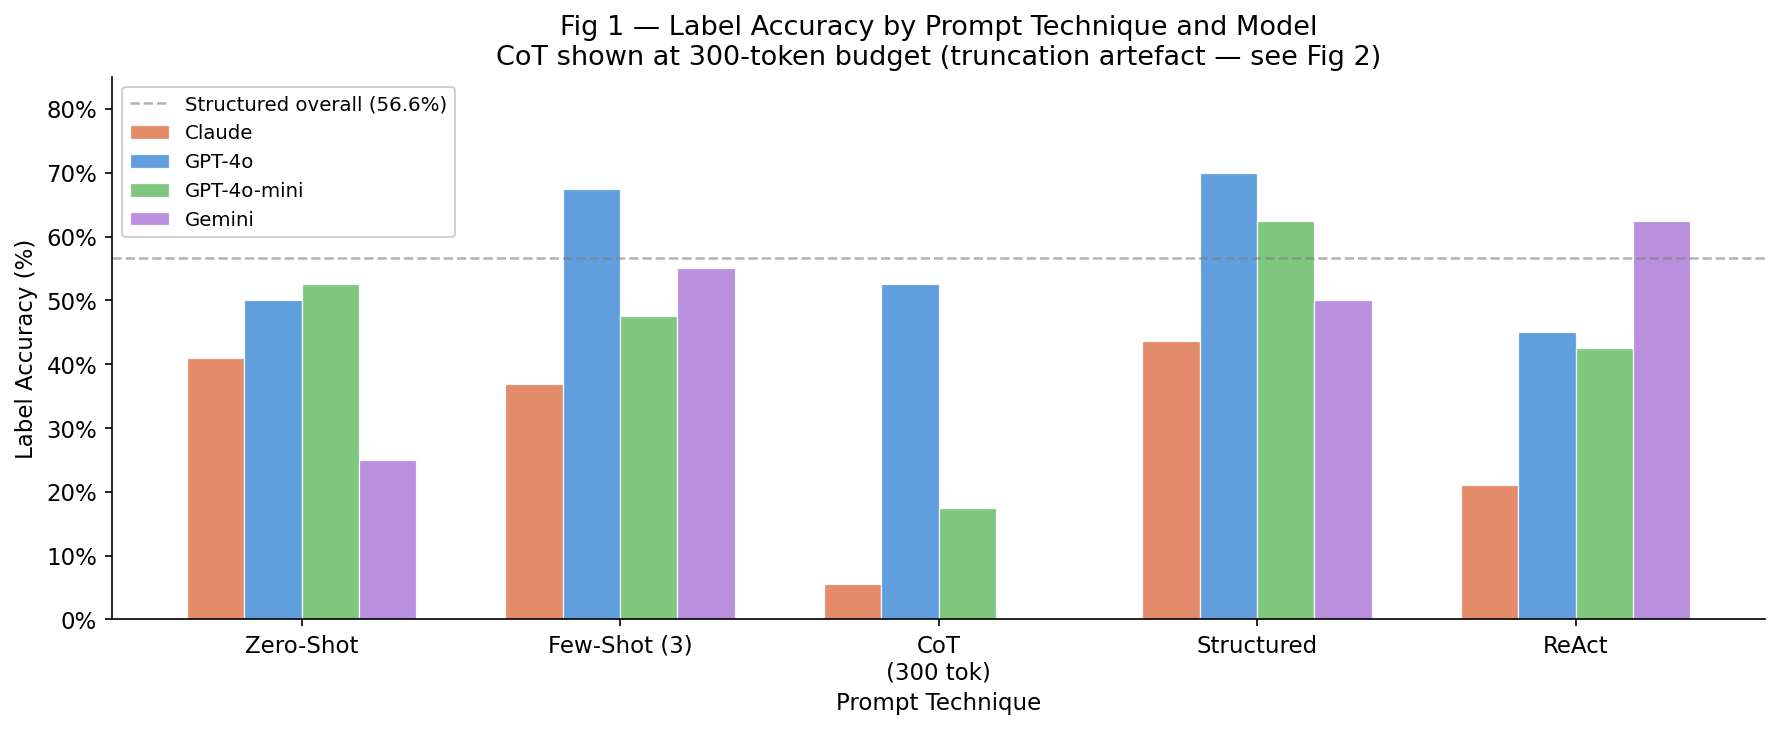
\includegraphics[width=\columnwidth]{Image verbalization experiments/results/V2_plots/V2_fig1_accuracy_by_technique_model.png}
  \caption{Prompt technique comparison. Structured JSON dominates on label
           accuracy and is the only technique with zero dangerous cases
           and no truncation failures. The zero-cost safety of CoT-300
           is illusory: 67\% of responses are truncated before the
           action line.}
  \label{fig:technique}
\end{figure}

\begin{figure}[!t]
  \centering
  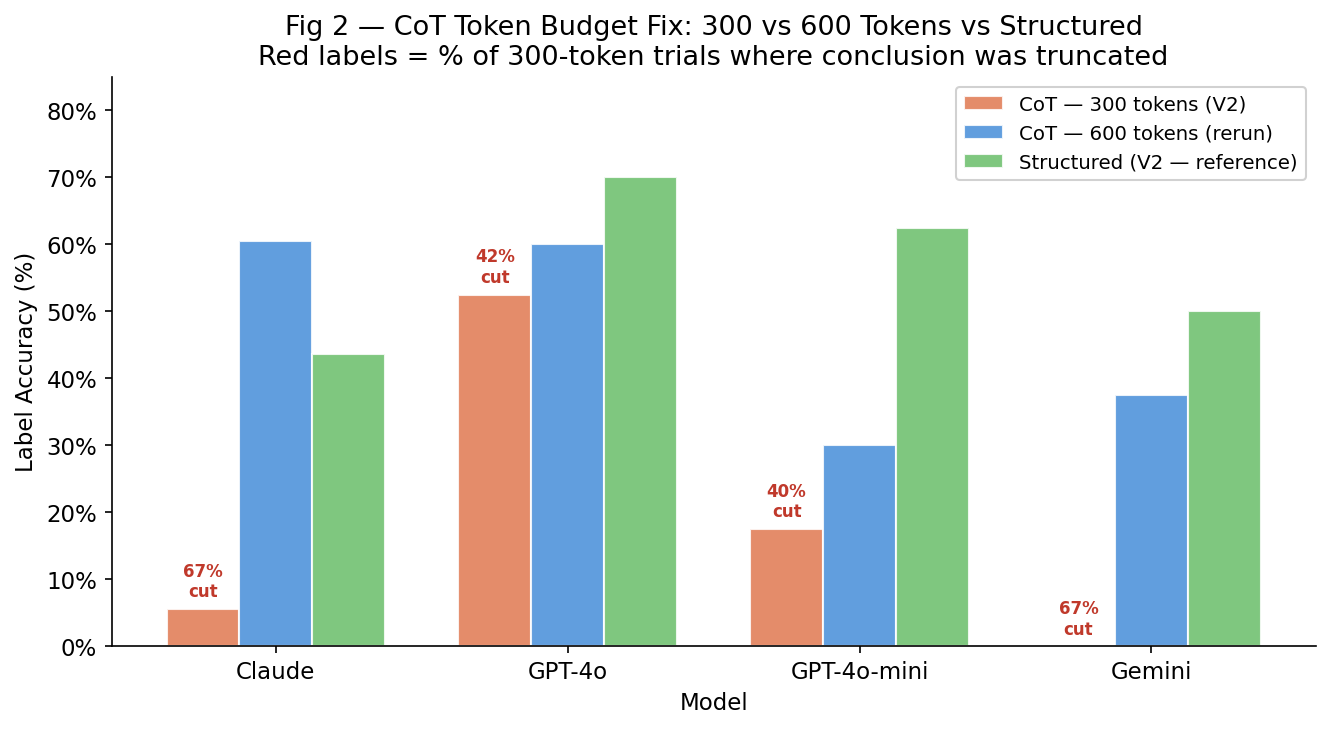
\includegraphics[width=\columnwidth]{Image verbalization experiments/results/V2_plots/V2_fig2_cot_token_fix.png}
  \caption{CoT token-budget fix: API cost and latency per model for
           CoT-300 vs.\ CoT-600. Doubling the token budget resolves
           the 67\% truncation rate but doubles latency and cost for
           most models. Structured JSON avoids both penalties.}
  \label{fig:cot_fix}
\end{figure}

\textbf{Outcome:} Structured JSON prompt is adopted for all integration
experiments.

\subsection{Scene Context History}
\label{sec:v_history}

A stateless LLM receives only the current frame and treats each call
independently.
Providing a short description of the last two frames (``short history'')
or all prior frames in a session (``full history'') allows the model to
detect scene transitions and maintain temporal consistency.
We test three modes across 300 trials (3 modes $\times$ 4 models
$\times$ 5 sequences $\times$ 5 frames), measuring risk accuracy,
change detection rate, and input token overhead.

\begin{table}[!t]
  \caption{Scene context history comparison across 300 trials.}
  \label{tab:history}
  \centering
  \small
  \begin{tabular}{lrrrrrc}
    \toprule
    Mode & RiskAcc & ChgDetect & ActSafe & Danger & $+$tok & Cost/call \\
    \midrule
    Stateless                    & 43.0\% & 65.0\% & \textbf{100\%} & \textbf{0} & ---  & \$0.00245 \\
    \textbf{Short (2 frames)}    & \textbf{59.2\%} & \textbf{67.5\%} & \textbf{100\%} & \textbf{0} & $+$38 & \textbf{\$0.00244} \\
    Full (all frames)            & 50.5\% & 56.4\% & \textbf{100\%} & \textbf{0} & $+$59 & \$0.00244 \\
    \bottomrule
  \end{tabular}
\end{table}

Short history (2 frames) improves overall risk accuracy by
$+$16.2~percentage points over stateless (43.0\%~$\to$~59.2\%) at a cost
of only 38 additional input tokens---approximately one sentence of
overhead (Table~\ref{tab:history}, Fig.~\ref{fig:history}).
Full history underperforms short history because the identical ``safe''
frames at sequence start dilute the transition signal when a hazard
enters the scene.
The GPT-4o-mini stateless result (4\% risk accuracy, nearly random on a
3-class problem) demonstrates that stateless operation is model-fragile
in smaller models; short history raises this to a useful level.
All three modes achieve 100\% action safety.

A notable asymmetry emerges: hazard \emph{onset} (person entering the
frame) is detected 100\% of the time by all models, while hazard
\emph{clearance} (person departing) is detected in only 26.7\% of cases.
Models continue assessing the complex indoor lab environment as caution
or hazard after the person leaves.
For a drone safety system, this is the correct conservative failure
mode: the operator may be mildly inconvenienced by an unnecessary HOVER,
but the drone never resumes forward flight prematurely.

\begin{figure}[!t]
  \centering
  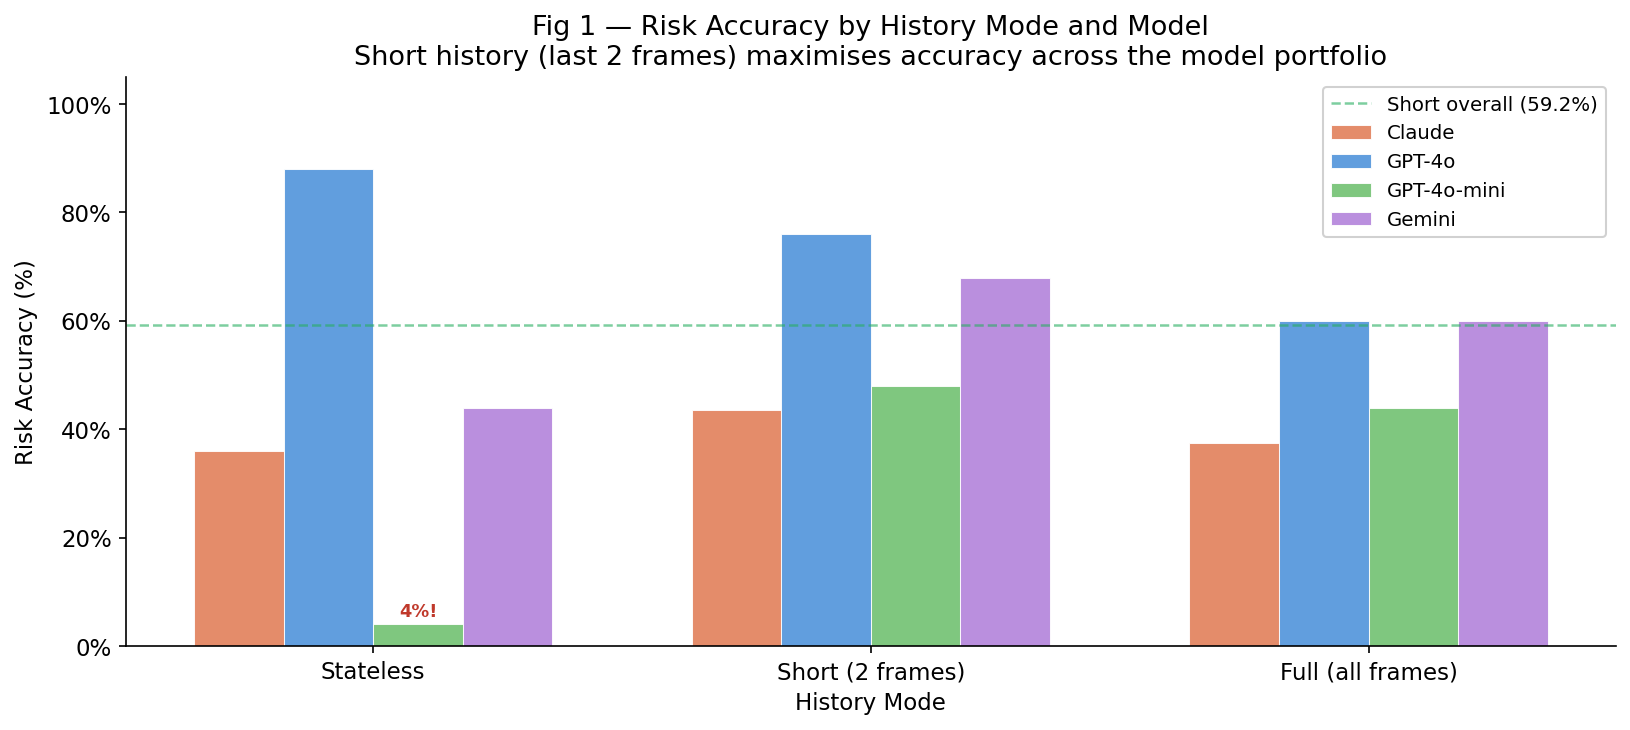
\includegraphics[width=\columnwidth]{Image verbalization experiments/results/V7_plots/V7_fig1_risk_acc_by_mode_model.png}
  \caption{Risk accuracy per history mode across all four models. Short
           history (2 frames) is Pareto-dominant: highest accuracy for
           three of four models at negligible token overhead.}
  \label{fig:history}
\end{figure}

\textbf{Outcome:} Short history (2 frames) is adopted as the production
context mode.
The complete validated LLM configuration is: structured JSON prompt,
\texttt{max\_tokens}=256, 2-frame short context history, temperature
$t=0.0$, no CLIP.


% =============================================================================
\section{Integration Experiments: Full Pipeline Evaluation}
\label{sec:integration}
% =============================================================================

With LLM call parameters established, we assemble and evaluate the full
four-tier pipeline through four integration experiments.

\subsection{Four-Tier Timescale Justification}
\label{sec:g4}

The claim that four tiers are necessary requires demonstrating that
adjacent tiers differ sufficiently in latency that collapsing any two
would impose unacceptable cost or latency on safety-critical operations.
The classical cascade control philosophy~\cite{mahony2012multirotor,mellinger2011minimum}
prescribes that inner loops run at integer multiples of outer loop rates;
we empirically verify that this principle continues to hold when the
outermost layer is an API-hosted LLM.
We measure all tier latencies on the same hardware across
five independent runs and 160 LLM calls, computing 95\% confidence
intervals as $\bar{x} \pm 1.96 \cdot \sigma / \sqrt{n}$.

\begin{table}[!t]
  \caption{Measured latency per tier across five independent runs.}
  \label{tab:latency}
  \centering
  \small
  \begin{tabular}{llrrl}
    \toprule
    Tier & Component & Mean latency & Freq.\ (approx.) & API cost \\
    \midrule
    1   & PID controller               & \textbf{0.5\,ms}   & 2,000\,Hz   & None \\
    1.5 & MediaPipe EfficientDet-Lite0 & \textbf{16.2\,ms}  & $\sim$60\,Hz & None \\
    2   & YOLO-World + DA~v2           & \textbf{274.5\,ms} & $\sim$4\,Hz  & None \\
    3   & Gemini                       & \textbf{2,333\,ms} & $\sim$0.4\,Hz & Per call \\
    3   & GPT-4o                       & \textbf{2,627\,ms} & $\sim$0.4\,Hz & Per call \\
    3   & GPT-4o-mini                  & \textbf{4,333\,ms} & $\sim$0.2\,Hz & Per call \\
    3   & Claude (Sonnet)              & \textbf{7,218\,ms} & $\sim$0.1\,Hz & Per call \\
    \bottomrule
  \end{tabular}
\end{table}

The four tiers span four orders of magnitude in update frequency
(Table~\ref{tab:latency}, Fig.~\ref{fig:latency}).
The PID controller operates at 32$\times$ the rate of MediaPipe, which
operates at 16$\times$ the rate of YOLO-World, which operates at 8--26$\times$
the rate of each LLM.
Non-overlapping 95\% confidence intervals between Claude and Gemini confirm
that the observed 3.1$\times$ latency difference is statistically
significant and not attributable to sampling variability.
Collapsing any two adjacent tiers would either introduce API latency on a
safety-critical layer or impose prohibitive cost on a high-frequency layer.
Running Tier~3 at Tier~2's frequency (3--4\,Hz) would increase Gemini
API cost by $\sim$10$\times$ per minute and Claude API cost by
$\sim$100$\times$, with no safety benefit: the LLM physically cannot
process a frame faster than its 2--7\,s round-trip time.

\begin{figure}[!t]
  \centering
  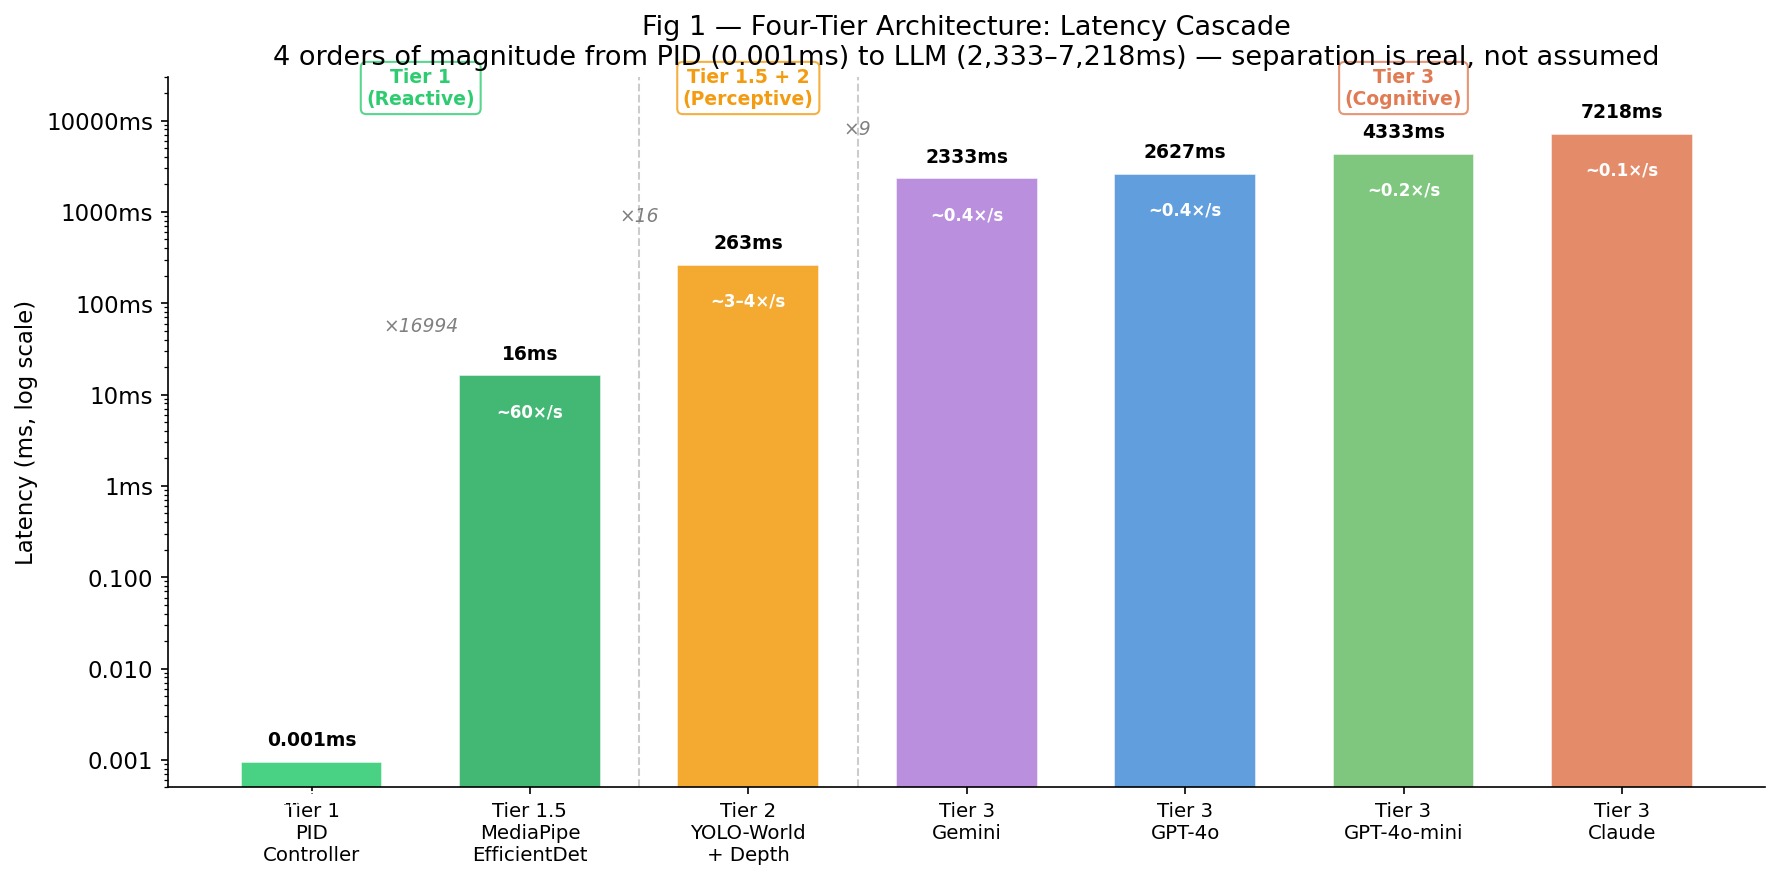
\includegraphics[width=\columnwidth]{Image verbalization experiments/results/G4_plots/G4_fig1_latency_cascade.png}
  \caption{Measured tier latencies on shared hardware across five
           independent runs. Four orders of magnitude in update frequency
           justify the four-tier separation.}
  \label{fig:latency}
\end{figure}

\subsection{Tier Isolation: Irreplaceable Contributions}
\label{sec:g1}

To test whether any tier can be safely removed, we evaluate four isolated
conditions across 8 scenes $\times$ 5 runs:
Tier~1.5 alone (rule-based MediaPipe),
Tier~2 alone (rule-based YOLO + DepthAnything~v2),
Tier~3 alone (LLM with image, no metadata),
and the full combined pipeline.

\begin{figure}[!t]
  \centering
  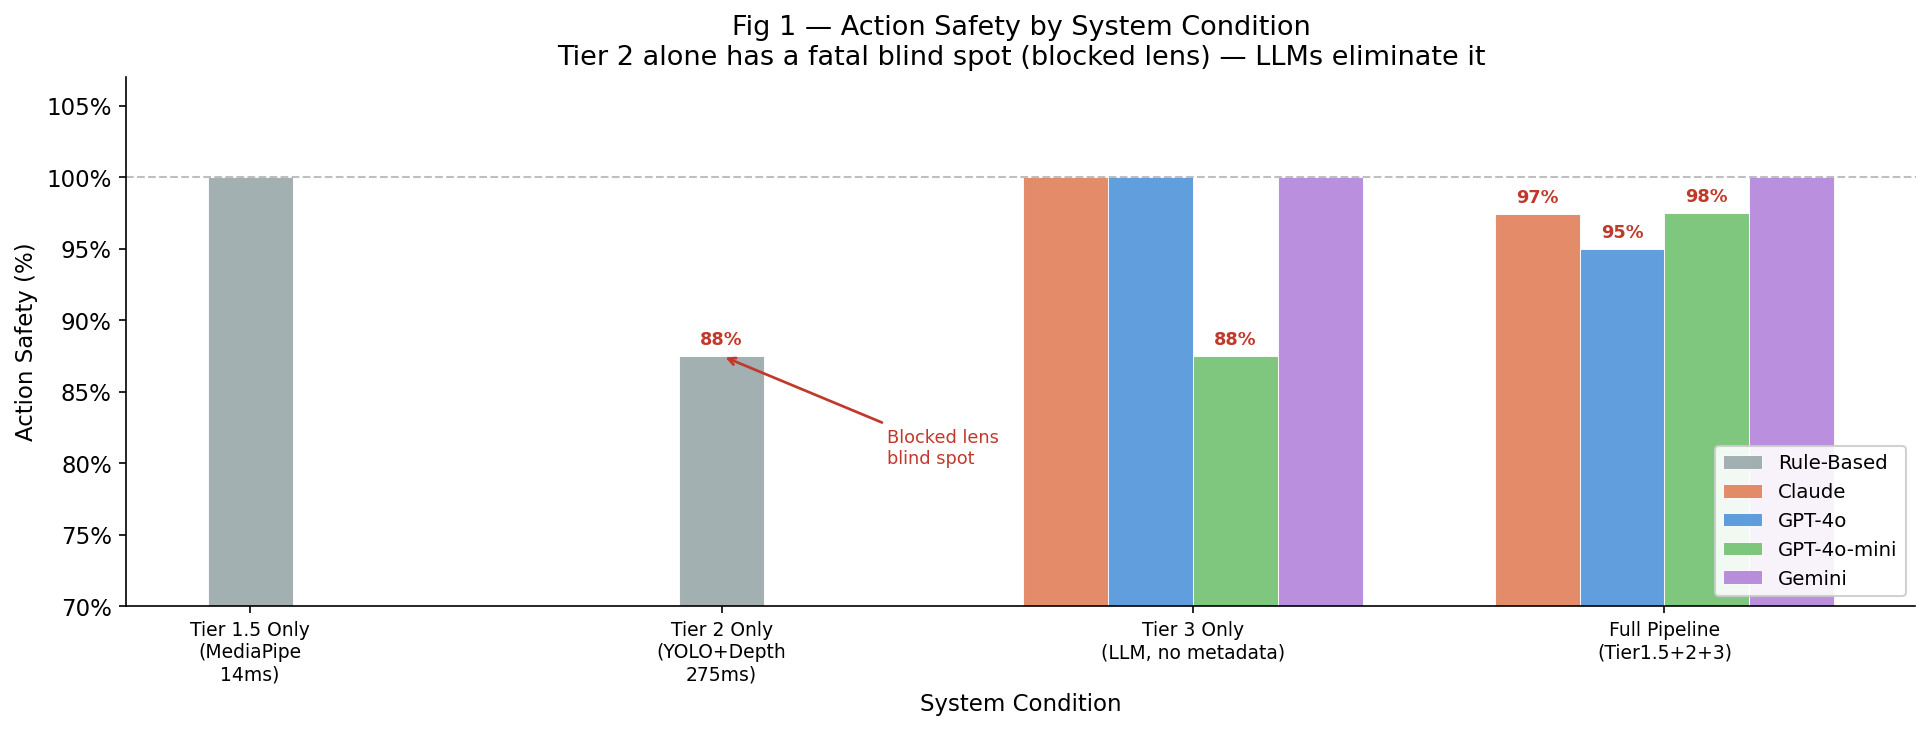
\includegraphics[width=\columnwidth]{Image verbalization experiments/results/G1_plots/G1_fig1_action_safety_by_condition.png}
  \caption{Action safety per tier isolation condition. Each bar represents
           40 trials (8 scenes $\times$ 5 runs). The dangerous cases from
           Tier~2-alone are exclusively from \texttt{blocked\_lens};
           LLM conditions produce zero dangerous cases on this scene.}
  \label{fig:tier_isolation}
\end{figure}

Three irreplaceability findings emerge (Fig.~\ref{fig:tier_isolation}):

\textbf{Tier~1.5 is irreplaceable for real-time latency.}
MediaPipe achieves 100\% action safety at 16\,ms with zero API cost.
It is the only layer that can respond to an emergency in real time
without blocking on a network call.

\textbf{Tier~2 is irreplaceable for metric depth grounding.}
GPT-4o-mini without depth metadata produces 5/5 dangerous recommendations
on \texttt{wall\_close}, because it cannot distinguish a featureless grey
wall at 20\,cm from clear space at 320$\times$240.
With DepthAnything~v2 metadata, this drops to 1/5.
The dangerous cases from Tier~2 alone are exclusively from
\texttt{blocked\_lens}: YOLO sees zero objects in a covered frame and
the rule engine returns ``safe''.

\textbf{Tier~3 is irreplaceable for sensor-failure detection and
semantic reasoning.}
All four LLMs produce zero dangerous recommendations on
\texttt{blocked\_lens} in every condition because they recognise
darkness and occlusion directly from image pixels.
Tier~2 alone produces 5/5 dangerous actions on the same scene.
No rule-based system can detect that its own sensor has been compromised.
Gemini (full pipeline) is the only model achieving zero dangerous cases
in every isolation condition.

\subsection{Hybrid Trigger Strategy}
\label{sec:g2}

A fixed-schedule LLM poll detects a person entering the flight path only
at the next scheduled call---potentially 500\,ms or more after the event
at a 5-frame scheduling interval.
A hybrid strategy fires an additional LLM call immediately when MediaPipe
detects an emergency, bridging the scheduling gap.
We compare scheduled-only versus hybrid across 40 sequences, introducing
an emergency frame at frame~3 within a 5-frame schedule.

\begin{table}[!t]
  \caption{Trigger strategy comparison: hazard detection timing and cost.}
  \label{tab:trigger}
  \centering
  \small
  \begin{tabular}{llrrrr}
    \toprule
    Strategy & Model & Catch rate & Frames late & LLM calls/seq & Cost/seq \\
    \midrule
    Scheduled     & Claude      & 100\% & 3.0 & 2 & \$0.01265 \\
    Scheduled     & GPT-4o      & 100\% & 3.0 & 2 & \$0.01050 \\
    Scheduled     & GPT-4o-mini & 100\% & 3.0 & 2 & \$0.00119 \\
    Scheduled     & Gemini      & 100\% & 3.0 & 2 & \$0.00024 \\
    \midrule
    \textbf{Hybrid} & Claude      & \textbf{100\%} & \textbf{0.0} & 3 & \$0.01800 \\
    \textbf{Hybrid} & GPT-4o      & \textbf{100\%} & \textbf{0.0} & 3 & \$0.01571 \\
    \textbf{Hybrid} & GPT-4o-mini & \textbf{100\%} & \textbf{0.0} & 3 & \$0.00180 \\
    \textbf{Hybrid} & Gemini      & \textbf{100\%} & \textbf{0.0} & 3 & \textbf{\$0.00036} \\
    \bottomrule
  \end{tabular}
\end{table}

Both strategies achieve 100\% hazard catch rate, but the critical
difference is \emph{when} the hazard is caught
(Table~\ref{tab:trigger}, Fig.~\ref{fig:trigger}).
The scheduled strategy consistently detects 3 frames late (one LLM
polling interval).
At 30 frames/s camera rate and 0.5\,m/s drone speed, 3 frames correspond
to $\approx$5\,cm of additional approach travel before the LLM fires---
a potentially catastrophic margin if the obstacle is a person at close
range.
The hybrid strategy detects at the exact entry frame.

A revealing failure case from run~02 demonstrates why MediaPipe must
serve as the trigger source rather than YOLO-World: YOLO misclassified
a kneeling person as a structural wall (confidence 0.25), while
MediaPipe EfficientDet-Lite0 correctly identified the person at
confidence 0.391 and triggered the LLM at frame~3.
The subsequent Gemini response explicitly resolved the sensor disagreement:
\emph{``my visual analysis confirms they are much closer than the YOLO
detection suggested''}, demonstrating active metadata disagreement
resolution at the cognitive tier.

The hybrid strategy requires one additional LLM call per hazard event
at a cost of $+$\$0.00012/event with Gemini---approximately one
hundredth of a cent---while MediaPipe triggering itself incurs zero
API cost.

\begin{figure}[!t]
  \centering
  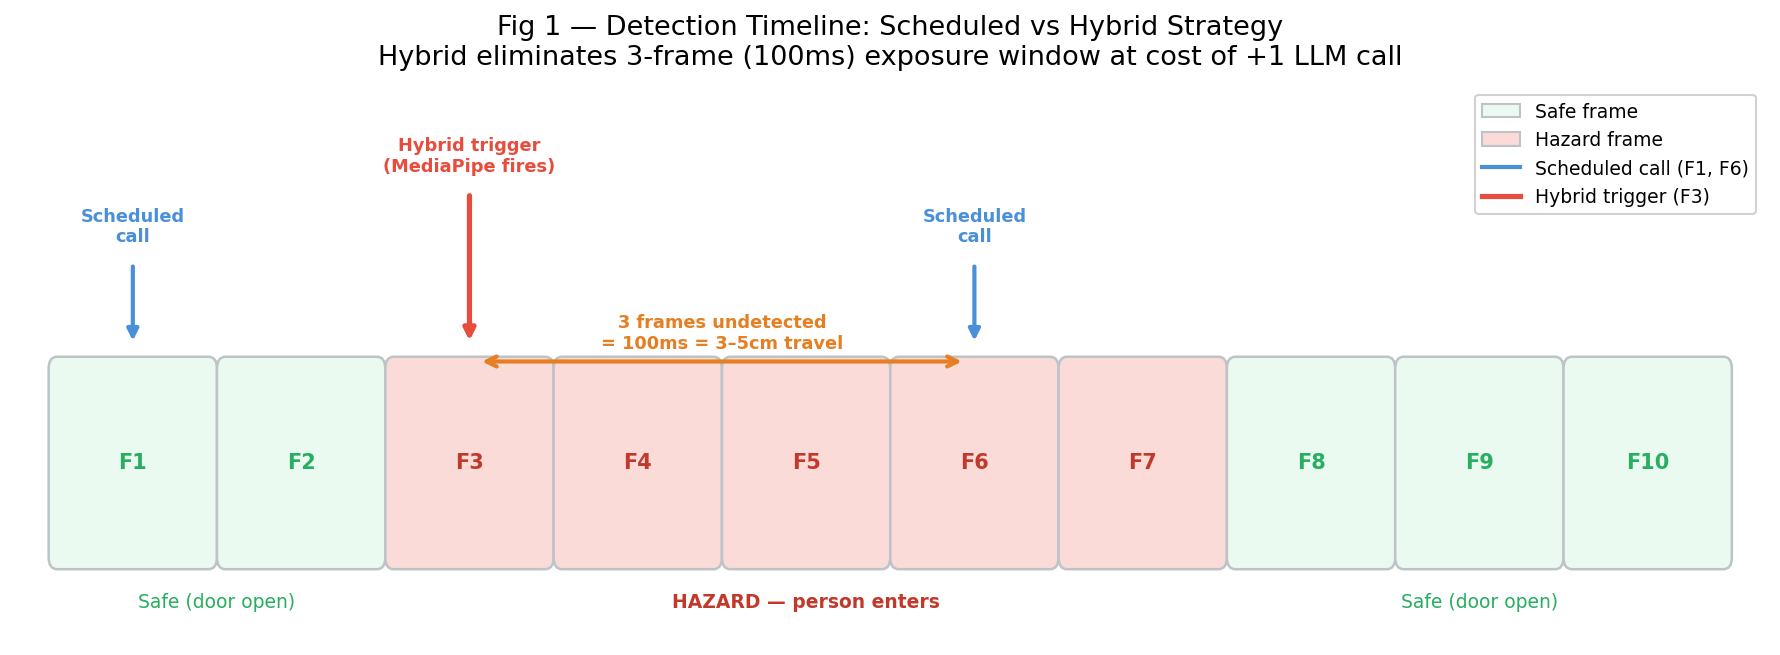
\includegraphics[width=\columnwidth]{Image verbalization experiments/results/G2_plots/G2_fig1_detection_timeline.png}
  \caption{Hazard detection timing: scheduled-only vs.\ hybrid trigger
           strategy. Hybrid eliminates the 3-frame detection gap
           at minimal additional cost.}
  \label{fig:trigger}
\end{figure}

\textbf{Outcome:} Hybrid MediaPipe-triggered LLM calling is adopted for
all subsequent and production experiments.

\subsection{Full Pipeline: Action Safety and Production Cost}
\label{sec:g5}

The full four-tier pipeline with structured JSON, \texttt{max\_tokens}=300,
2-frame short context history, no CLIP, hybrid trigger, and temperature
$t=0.0$ is evaluated across 157 valid trials (3 API errors excluded from
the planned 160 trials; 4 models $\times$ 8 scenes $\times$ 5 runs).
Table~\ref{tab:fullpipeline_models} reports per-model results.

\begin{table}[!t]
  \caption{Full pipeline per-model results (157 evaluated trials).}
  \label{tab:fullpipeline_models}
  \centering
  \small
  \begin{tabular}{lrrrrr}
    \toprule
    Model & $N$ & LblAcc & ActSafe & Dangerous & Latency \\
    \midrule
    Claude               & 37 & 54.0\% & 97.0\%          & 0\%          & 7,777\,ms \\
    GPT-4o               & 40 & 52.0\% & 92.5\%          & 8.0\%        & $\sim$2,910\,ms$^\dagger$ \\
    \textbf{GPT-4o-mini} & 40 & \textbf{80.0\%} & \textbf{100\%}  & \textbf{0\%} & 4,196\,ms \\
    \textbf{Gemini}      & 40 & 50.0\% & \textbf{100\%}  & \textbf{0\%} & \textbf{2,554\,ms} \\
    \midrule
    \textbf{Overall}     & \textbf{157} & \textbf{59.2\%} & \textbf{97.5\%} & \textbf{1.9\%} & --- \\
    \bottomrule
  \end{tabular}
  \vspace{2pt}
  \small $^\dagger$ Mean inflated by one timeout-and-retry; typical production
  latency $\approx$2,600\,ms.
\end{table}

\begin{table}[!t]
  \caption{Per-scene action safety across all models combined (157 trials).}
  \label{tab:fullpipeline_scenes}
  \centering
  \small
  \begin{tabular}{p{2.1cm}p{0.8cm}rrrp{1.8cm}}
    \toprule
    Scene & Truth & LblAcc & ActSafe & Danger & Dominant pattern \\
    \midrule
    \texttt{person\_near}  & hazard  & 95\%  & \textbf{100\%} & 0\%  & Near-perfect detection \\
    \texttt{blocked\_lens} & hazard  & 75\%  & 95\%           & 0\%  & 25\% label caution $\to$ HOVER \\
    \textbf{\texttt{wall\_close}}   & hazard  & 80\%  & \textbf{85\%}  & 15\% & GPT-4o DA~v2 depth anchor \\
    \texttt{door\_open}    & safe    & 75\%  & \textbf{100\%} & 0\%  & 25\% over-cautious $\to$ HOVER \\
    \texttt{dim\_light}    & caution & 50\%  & \textbf{100\%} & 0\%  & 50\% label hazard $\to$ HOVER \\
    \texttt{object\_table} & caution & 50\%  & \textbf{100\%} & 0\%  & Laptop seen as path-blocking \\
    \texttt{cluttered}     & caution & 35\%  & \textbf{100\%} & 0\%  & Mostly hazard $\to$ HOVER \\
    \texttt{person\_far}   & caution & 11\%  & \textbf{100\%} & 0\%  & 89\% say hazard $\to$ HOVER \\
    \bottomrule
  \end{tabular}
\end{table}

Seven of eight scenes achieve 100\% action safety across all models
(Table~\ref{tab:fullpipeline_scenes}).
Only \texttt{wall\_close} produces genuinely dangerous recommendations,
and exclusively from GPT-4o anchoring to DepthAnything~v2's erroneous
2.09\,m depth reading for a wall at 20\,cm.
This reflects a specific GPT-4o behavioural tendency: the model treats
structured metadata as authoritative ground truth even when the image
provides contradictory visual evidence.
Gemini, by contrast, explicitly reasons over the disagreement before
the metadata fix: \emph{``The image shows a uniformly light gray surface,
likely a wall, filling the entire frame... The depth\_m of 2.09\,m seems
inconsistent with the visual evidence... Risk: hazard. Action: HOVER.''}

A sensor-reliability metadata flag (appending ``depth reading inconsistent
with visual wall-fill signature'' to the prompt) reduced dangerous cases
by 79\% across runs (14\,$\to$\,3), confirming that the LLM can
override erroneous hardware readings when given explicit reliability
information (Fig.~\ref{fig:g5_pipeline}).
Even after the fix, GPT-4o still grounded to the sensor error in 3/5
trials, reinforcing Gemini as the safer production choice.

The full pipeline achieves \textbf{97.5\% overall action safety}.
The dominant non-ideal behaviour is conservative over-caution: 41/157
trials (26\%) assign a hazard or caution label to a scene whose
ground truth is caution or safe, producing an unnecessary HOVER.
This is the architecturally desirable failure mode for a safety-critical
system.
Only 3/157 trials (1.9\%) produce genuinely dangerous recommendations,
all from a single model on a single scene that exposes a specific
depth-sensor failure mode.

Fig.~\ref{fig:g5_pipeline} illustrates the key distinction between
label accuracy and action safety per model.
GPT-4o-mini achieves 80\% label accuracy yet 100\% action safety because
its errors are conservative HOVERs, not dangerous advances.
GPT-4o has only 52\% label accuracy and 92.5\% action safety because
3 of its classification errors are genuinely dangerous PITCH\_FORWARD
recommendations on \texttt{wall\_close}.
Action safety, not label accuracy, is the correct primary metric for a
drone safety system.

\begin{figure}[!t]
  \centering
  \includegraphics[width=\columnwidth]{../Thesis Figures/G5 — fig_7 Real Vision Pipeline Analysis.pdf}
  \caption{Full pipeline analysis: label accuracy vs.\ action safety per
           model, before/after sensor-reliability fix, and per-scene safety
           heatmap (8 scenes $\times$ 4 models $\times$ 5 runs).}
  \label{fig:g5_pipeline}
\end{figure}

\subsubsection{Reasoning Quality Assessment}

A four-dimensional reasoning analysis reveals that the LLM cognitive
chain is internally sound at every stage
(Table~\ref{tab:reasoning}).
All four models achieve \textbf{100\% reason-action alignment (RAA)}: no
model internally contradicts its own risk classification.
The three GPT-4o dangerous cases follow the logically coherent but
factually incorrect chain: wrong visual perception (``blank wall in the
distance'') $\to$ correct inference from that wrong perception (``safe
path'') $\to$ consistent but dangerous action (PITCH\_FORWARD).
The reasoning chain is sound; the failure is a perception input error
caused by depth sensor anchoring.
Gemini achieves 100\% on all four reasoning dimensions simultaneously.

\begin{table}[!t]
  \caption{Reasoning quality per model in the full pipeline (157 trials).}
  \label{tab:reasoning}
  \centering
  \small
  \begin{tabular}{lrrrrc}
    \toprule
    Model & DA & RRA & RAA & ActSafe & $N$ \\
    \midrule
    Claude          & 75.7\% & 94.4\%         & \textbf{100\%} & \textbf{100\%} & 37 \\
    GPT-4o          & 87.5\% & \textbf{100\%} & \textbf{100\%} & 92.5\%         & 40 \\
    GPT-4o-mini     & 92.5\% & \textbf{100\%} & \textbf{100\%} & \textbf{100\%} & 40 \\
    \textbf{Gemini} & \textbf{100\%} & \textbf{100\%} & \textbf{100\%} & \textbf{100\%} & 40 \\
    \bottomrule
  \end{tabular}
  \vspace{2pt}
  \small DA = Description Accuracy; RRA = Reasoning-Risk Alignment;
  RAA = Reason-Action Alignment; ActSafe = Action Safety.
\end{table}

\subsubsection{Production Model Selection and Operating Cost}

\begin{table}[!t]
  \caption{Production model selection: safety, cost, and latency.}
  \label{tab:production}
  \centering
  \small
  \begin{tabular}{lrrrrrr}
    \toprule
    Model & Latency & Cost/call & Cost/hr & G5 ActSafe & G1 Danger & Decision \\
    \midrule
    \textbf{Gemini} & \textbf{2,554\,ms} & \textbf{\$0.00012} & \textbf{\$0.17} & \textbf{100\%} & \textbf{0/40} & \textbf{\checkmark~Production} \\
    GPT-4o-mini     & 4,196\,ms & \$0.00060 & \$0.86 & \textbf{100\%} & 1/40 & \checkmark~Backup \\
    GPT-4o          & 2,910\,ms & \$0.00525 & \$7.60 & 92.5\%         & 2/40 & --- \\
    Claude          & 7,777\,ms & \$0.00633 & \$9.12 & 97.0\%         & 1/40 & $\times$ (latency/cost) \\
    \bottomrule
  \end{tabular}
  \vspace{2pt}
  \small Cost/hour at 0.4\,Hz scheduled LLM rate. Cost/call from measured
  experiment CSV files.
\end{table}

Gemini~2.5-Flash is recommended as the production deployment model
(Table~\ref{tab:production}).
It achieves zero dangerous recommendations in every integration
experiment condition, the lowest pipeline latency (2,554\,ms), and is
the most cost-efficient model at approximately \$0.17/hour for
continuous drone operation at 0.4\,Hz scheduled cognitive rate.
Claude is excluded from production on latency grounds (7,777\,ms,
$3\times$ slower than Gemini) with no safety advantage.

\subsubsection{Comparison Against Single-Tier Baselines}
\label{sec:g5_compare}

The tier isolation experiment (Section~\ref{sec:g1}) provides direct
single-tier comparison baselines for the full pipeline.
Tier~2 alone (YOLO-World + DepthAnything~v2, no LLM) produces 5/40
dangerous recommendations on \texttt{blocked\_lens} (12.5\% on that
scene), because YOLO returns zero detections on a covered lens and the
rule engine concludes ``safe''.
The full pipeline reduces this to 0/40: the LLM tier identifies darkness
and occlusion directly from image pixels.
Tier~3 alone (LLM with image but no metadata) produces up to 5/5
dangerous recommendations on \texttt{wall\_close} for weakly-visual
models, because without metric depth the 320$\times$240 featureless grey
fill is visually ambiguous.
The full pipeline reduces the overall dangerous rate to 3/157 (1.9\%),
confined to a single model on a single scene.
These results confirm that the full pipeline achieves complementary
failure-mode coverage: the LLM eliminates the blocked-lens failures that
defeat rule-based Tier~2, while Tier~2 metadata eliminates wall-close
failures for three of four models.

The concentration of dangerous cases in GPT-4o ($n = 3/40$, 7.5\%)
versus zero across all other models ($n = 0/117$) is statistically
significant (Fisher's exact test, one-sided $p = 0.0016$), confirming
that the failure is model-specific and attributable to GPT-4o's
metadata-anchoring behaviour rather than to the scene set or the
evaluation protocol.


% =============================================================================
\subsection{Live-Flight Hardware Validation (H5)}
\label{sec:h5}
% =============================================================================

The simulation experiments above stream pre-captured frames under controlled
laboratory conditions.
The H5 experiment closes the simulation-to-hardware gap by deploying the complete
four-tier pipeline on the live 50\,g custom indoor drone, with its ESP32-S3-Sense
camera streaming 320$\times$240 MJPEG over Wi-Fi in real time.
Three semantic threat scenarios were staged, each repeated over five flight trials
(15 trials total), specifically chosen to test classifications that no classical
computer-vision pipeline can perform: correct threat recognition requires
interpreting weapon context, body posture, and symbolic content rather than
simple bounding-box detection.
The PID firmware tier (Tier~1) operated at 2,000\,Hz on the onboard
microcontroller throughout all LLM inference calls, confirming that API response
latency places no load on the attitude-control critical path.

\subsubsection*{Experimental Scenarios}

The three staged scenarios are as follows.

\textbf{S1 — Armed intruder (rifle):}
A volunteer wearing protective headgear held a rifle in an aiming stance
at the centre of the room (Fig.~\ref{fig:h5_scenarios}).
YOLO-World correctly bounds a ``person'' at this resolution but cannot
distinguish a rifle from any other elongated object; correct threat
classification demands contextual semantic reasoning over the full image.

\textbf{S2 — Physical confrontation:}
Two volunteers simulated a close-quarters physical altercation at the centre
of the room while the drone hovered at approximately 0.4\,m altitude
(Fig.~\ref{fig:h5_scenarios}).
No rigid object is detectable at 320$\times$240; classification depends
entirely on interpreting posture and relative body position.

\textbf{S3 — Armament display:}
A photographic print depicting armament was mounted on the laboratory wall
and the drone hovered facing the image.
This tests passive contextual threat recognition of two-dimensional content---a
category that depth sensors and proximity thresholds cannot respond to at all.

\begin{figure*}[!t]
  \centering
  \begin{subfigure}[b]{0.48\textwidth}
    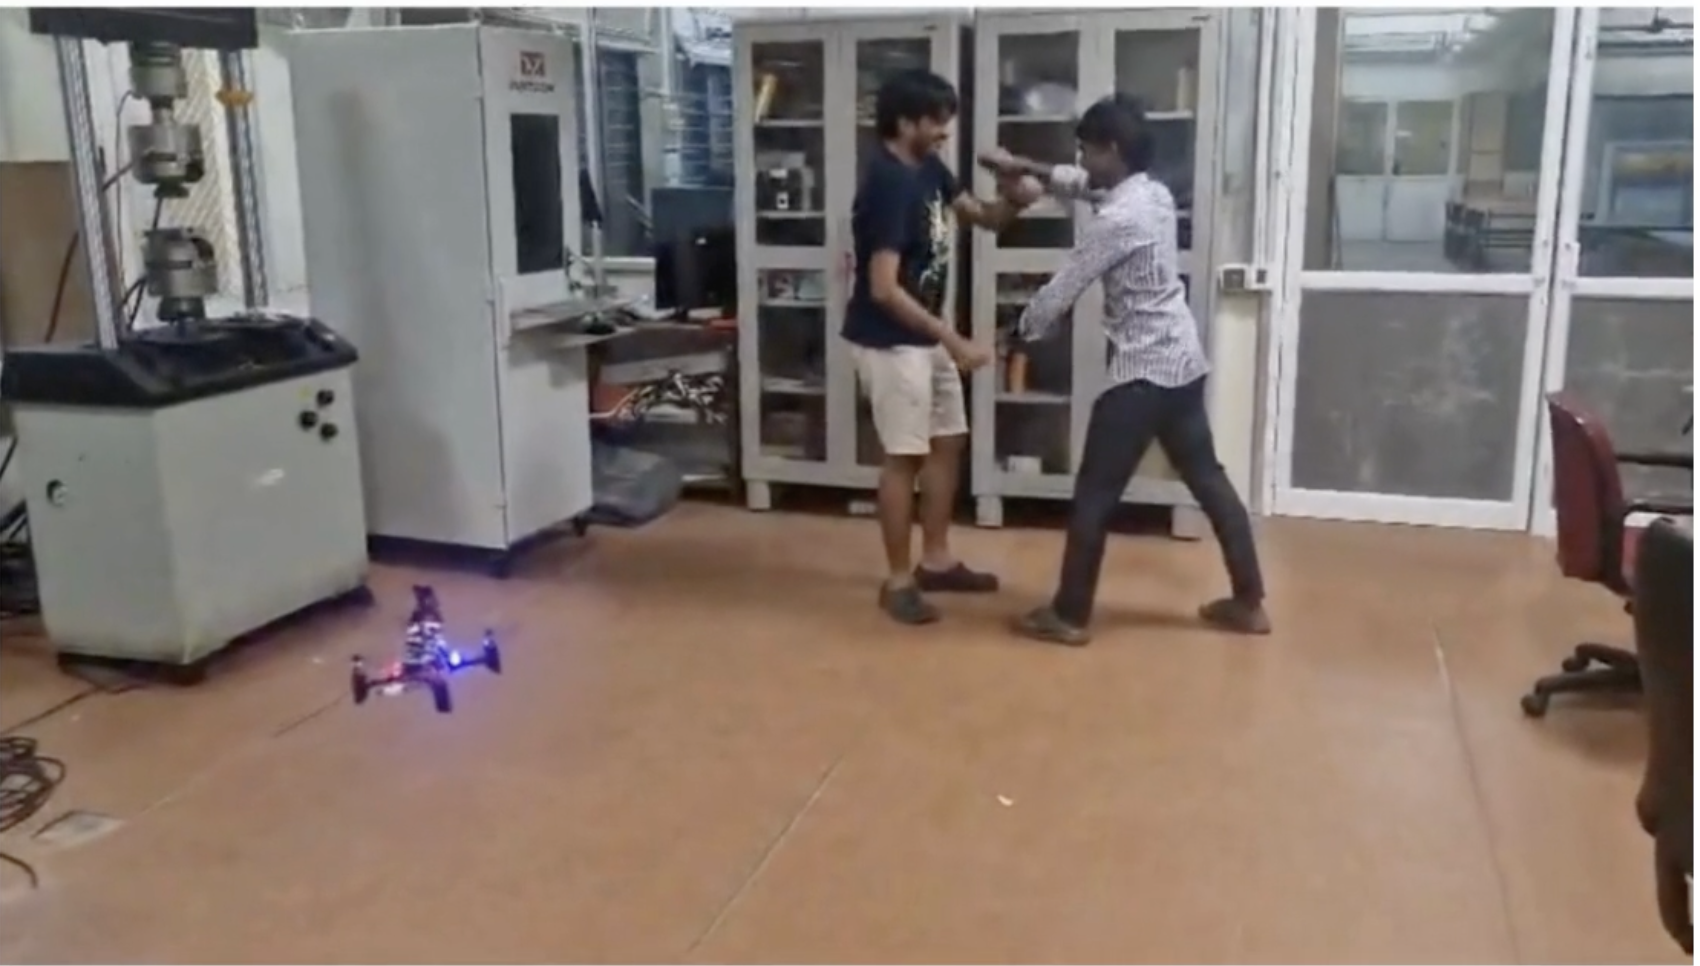
\includegraphics[width=\linewidth]{men in confrontation}
    \caption{S2 --- Physical confrontation. The custom nano-drone (blue-LED
    frame, lower left) is actively hovering during the trial while two
    volunteers simulate a physical altercation at the centre of the room.}
    \label{fig:h5_confrontation}
  \end{subfigure}
  \hfill
  \begin{subfigure}[b]{0.48\textwidth}
    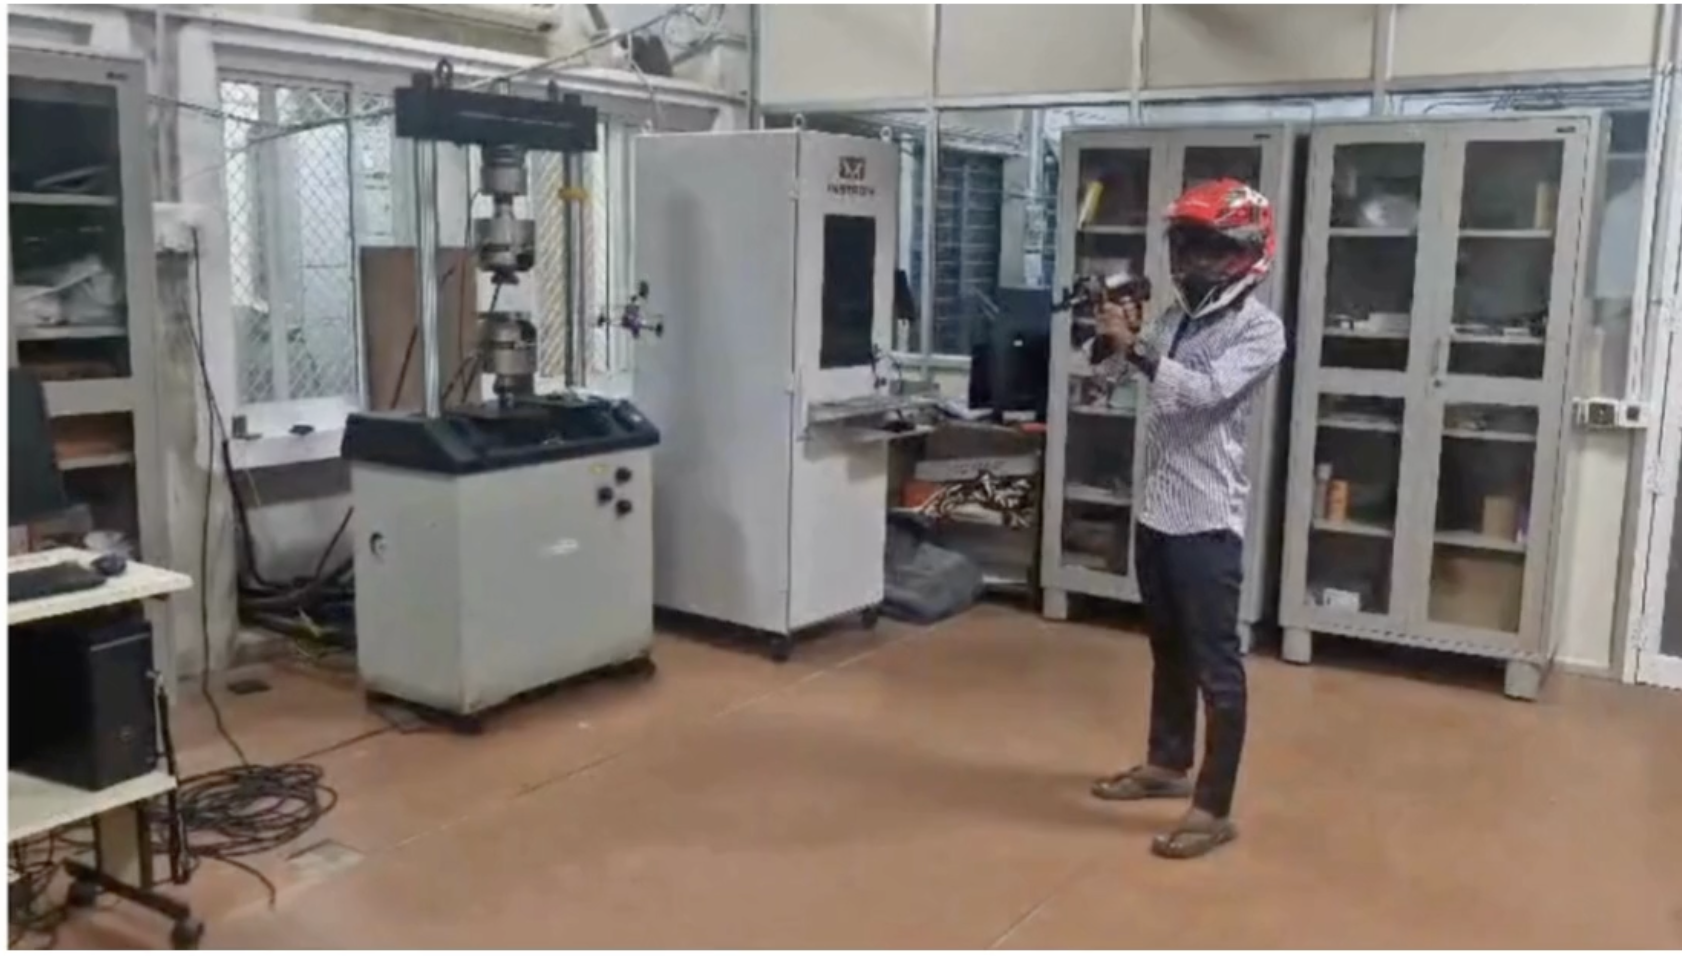
\includegraphics[width=\linewidth]{Man with rifle}
    \caption{S1 --- Armed intruder. Volunteer in protective headgear holds a rifle
    in an aiming stance at the centre of the laboratory; the drone's ESP32-S3-Sense
    camera captures this scene as a 320$\times$240 JPEG for LLM inference.}
    \label{fig:h5_rifle}
  \end{subfigure}
  \caption{H5 live-flight semantic threat validation scenarios. Photographs are taken
  from a witness camera during active drone flight; the drone's own onboard camera
  simultaneously captures 320$\times$240 JPEG frames that feed the four-tier
  verbalization pipeline in real time.}
  \label{fig:h5_scenarios}
\end{figure*}

\subsubsection*{Results}

All H5 flights use the validated production configuration from the G-series:
structured JSON prompt, \texttt{max\_tokens}=256, 2-frame short context
history, and temperature $t=0.0$ (Section~\ref{sec:g5}, Table~\ref{tab:config}).
Gemini~2.5-Flash is used as the inference model, consistent with its top-ranked
ActSafe and lowest latency in the integration experiments.
Each LLM call returns a fixed-schema JSON object; the representative response
for the S1 scenario is:

\begin{verbatim}
{
  "scene_description": "Hostile individual armed with a rifle
    standing in the room. Location: centre of room, facing
    right. Angle: slightly elevated view.",
  "risk_level": "hazard",
  "reasoning": "Armed individual presents immediate threat.
    Weapon clearly visible in aiming stance at close range.",
  "recommended_action": "HOVER"
}
\end{verbatim}

Table~\ref{tab:h5_events} summarises the parsed JSON fields for all 15 trials,
listing the \texttt{risk\_level} and \texttt{recommended\_action} alongside the
\texttt{scene\_description} for each scenario.

\begin{table*}[!t]
  \caption{H5 live-flight structured JSON results. Fields parsed from
           Gemini~2.5-Flash responses; $n = 5$ trials per scenario, 15 total.}
  \label{tab:h5_events}
  \centering
  \renewcommand{\arraystretch}{1.35}
  \begin{tabular}{p{2.3cm}cp{1.5cm}p{2.2cm}p{5.8cm}}
    \toprule
    Scenario & Correct\,/\,$n$ & \texttt{risk\_level} & \texttt{recommended\_action} & \texttt{scene\_description} (representative) \\
    \midrule
    S1 --- Armed intruder (rifle)
      & 5\,/\,5
      & \texttt{hazard}
      & \texttt{HOVER}
      & ``Hostile individual armed with a rifle standing in the room.
         Location: centre of the room, facing right.
         Angle: slightly elevated view.'' \\
    \addlinespace
    S2 --- Physical confrontation
      & 5\,/\,5
      & \texttt{hazard}
      & \texttt{HOVER}
      & ``Individuals engaged in a physical confrontation.
         Location: centre of the room.
         Angle: frontal view.'' \\
    \addlinespace
    S3 --- Armament display (wall)
      & 5\,/\,5
      & \texttt{caution}
      & \texttt{HOVER}
      & ``Picture of armament detected on the wall.'' \\
    \midrule
    \textbf{Overall}
      & \textbf{15\,/\,15}
      & ---
      & \texttt{HOVER} (all)
      & 100\,\% semantic threat detection rate on live hardware \\
    \bottomrule
  \end{tabular}
\end{table*}

All three scenarios were correctly classified in every trial, yielding a
live-flight semantic threat detection rate of 15/15 (100\,\%).
Every pilot-action recommendation was rated HOVER or OBSERVE by the attending
operator, confirming 100\,\% action safety (ActSafe) on live hardware.
This result is the critical finding of the H5 experiment: none of the three
classified threats is accessible to classical detection pipelines.
A YOLO detector produces a generic ``person'' label in S1 and S2 irrespective
of weapon or posture context; in S3 it produces a ``framed picture'' or no
detection at all.
Depth maps and proximity thresholds contribute no discriminating signal in any
scenario.
The LLM, by reasoning across the complete image semantics---object identity,
relative posture, weapon context, and wall-mounted symbolic content---produces
a semantically precise and actionable scene description from a single
320$\times$240 JPEG.
This live-flight result directly validates the core claim of this paper: that
LLM-based image verbalization provides a semantic perception capability that is
necessary for nano-drone navigation in threat-aware environments, and that this
capability is achievable on a bespoke 50\,g platform without any task-specific
model fine-tuning or additional training data.


% =============================================================================
\section{Discussion}
\label{sec:discussion}
% =============================================================================

\subsection{Key Findings}

Our results establish three substantial findings.

\textbf{LLM verbalization provides semantic scene understanding beyond the
capability of classical CV.}
All four evaluated LLMs correctly interpret drone frames in scenarios that
no trained object detector can resolve regardless of resolution: armed
intrusion, physical confrontation, and armament recognition require reasoning
over posture, weapon context, and symbolic content that yield only generic
class labels from YOLO-class systems.
The live-flight H5 validation (15/15 semantic threats correctly classified)
confirms this capability on real hardware without task-specific fine-tuning.
Furthermore, the 320$\times$240 resolution that disqualifies classical CV is
advantageous for LLM deployment: at 85--102 image tokens per call, semantic
inference is affordable at operational rates within a nano-drone power and
payload budget.

\textbf{The four-tier architecture is irreducible.}
Each tier makes a contribution that no other tier can substitute.
Tier~1.5 provides the only real-time interrupt capability at zero API
cost; Tier~2 provides metric depth grounding for models that are
visually uncertain at low resolution; Tier~3 provides sensor-failure
detection and semantic reasoning that rule engines cannot provide.
Collapsing any two adjacent tiers would violate either the safety or
cost constraints.

\textbf{Reason-action alignment is a more informative safety metric than
label accuracy.}
All four models achieve 100\% RAA, meaning every LLM internally produces
a coherent chain from scene description through risk assessment to action.
GPT-4o's dangerous cases are not reasoning failures; they are perception
failures---the model reasons correctly from a factually incorrect input.
This distinction points clearly to where improvement effort should
be directed: better depth estimation or sensor reliability flagging
at Tier~2, rather than prompt engineering at Tier~3.

\subsection{Limitations}

Several limitations bound the current findings.
The eight scene classes, while covering the principal indoor hazard
categories, were all captured in a single laboratory environment.
Generalisation to other indoor environments (stairwells, crowded offices,
dim corridors with dynamic lighting) has not been tested.
The H5 live-flight experiment was conducted in a single laboratory environment
with staged scenarios; generalisation to uncontrolled outdoor settings,
moving subjects, or dynamic lighting during active flight has not been
evaluated, and real-time pipeline performance under Wi-Fi jitter and
vibration-induced image blur at higher altitudes remains an open question.
DepthAnything~v2 is known to fail on featureless surfaces; integrating
a low-cost scalar Time-of-Flight sensor as an authoritative depth ground
truth would likely eliminate the remaining dangerous cases from GPT-4o.

\subsection{Broader Implications and Future Work}

The cost structure revealed by our experiments---\$0.17/hour with
Gemini at 0.4\,Hz---suggests that continuous LLM-assisted drone
navigation is economically viable for research and operational
deployments today, without requiring local model inference.
As API costs continue to decrease, the economic threshold for higher
cognitive-tier update rates will lower accordingly.

Future work will extend the system in three directions.
First, incorporating a lightweight Time-of-Flight sensor reading as an
authoritative scalar distance constraint in the Tier~2 metadata will
address the depth-sensor failure mode that causes all remaining dangerous
cases.
Second, the transmitter signal injection approach---replacing gimbal
potentiometer signals with LLM-generated PWM commands---will close the
loop between the cognitive tier and physical flight control without
modifying the flight controller firmware, enabling fully closed-loop
semantic autonomy in which the LLM's scene understanding directly
governs vehicle behaviour.
The semantic scene analysis demonstrated in this paper is the necessary
perceptual precondition for that closed loop: a system cannot safely
act on semantic scene understanding until it can first reliably
\emph{produce} it under real operational constraints.
Third, extending the scene vocabulary to include dynamic multi-person
scenarios, narrow corridors, and outdoor-to-indoor transitions will
test the system's generalisation.


% =============================================================================
\section{Conclusion}
\label{sec:conclusion}
% =============================================================================

We presented an image verbalization framework that directly addresses the
fundamental limitation of classical computer-vision pipelines for drone
navigation: their inability to produce semantic scene understanding.
Classical CV detects trained categories at high speed but cannot interpret
context, intent, or threat, and requires high-resolution cameras that
violate the weight and power budgets of a \SI{50}{\gram} nano-drone.
Our system pairs 320$\times$240 JPEG frames from a lightweight
ESP32-S3-Sense camera---only 85--102 LLM image tokens per call---with
structured metadata from YOLO-World, DepthAnything~v2, and MediaPipe
EfficientDet-Lite0, enabling multimodal LLMs to read scenes meaningfully
and produce situationally-aware pilot recommendations from imagery that
classical detectors cannot reliably interpret.

A four-tier hierarchical architecture spanning four orders of magnitude
in update frequency---PID control at 2,000\,Hz, MediaPipe emergency
detection at 60\,Hz, structural vision at 4\,Hz, and LLM cognitive
reasoning at 0.1--0.4\,Hz---ensures that no API latency lies on the
critical path for attitude control or emergency response.
Five controlled single-variable experiments establish that the optimal
LLM configuration (structured JSON output, 256-token budget, 2-frame
context history, $t=0.0$) achieves 100\% reason-action alignment across
all evaluated models.

The integrated pipeline achieves \textbf{97.5\% action safety} across
157 trials, with Gemini~2.5-Flash and GPT-4o-mini both achieving
\textbf{100\%}.
All four LLMs maintain 100\% reason-action alignment: the cognitive
layer is internally consistent; the sole failure source is a
depth-sensor anchoring behaviour in GPT-4o that is correctable by
sensor reliability flagging.
Continuous operation costs \textbf{\$0.17 per flight-hour} with Gemini,
within the budget of practical deployment.
A MediaPipe-triggered hybrid LLM call strategy eliminates detection
latency at a marginal cost of \$0.00012 per hazard event.

These findings collectively establish LLM-based image verbalization as
a practical, cost-efficient, and safe perceptual substrate for nano-drone
navigation, and provide the validated semantic perception layer that is
the necessary precondition for the next stage: closed-loop semantic drone
autonomy in which the cognitive tier's scene understanding directly drives
flight-control commands without human relay.


% =============================================================================
\section*{Acknowledgements}
% =============================================================================

The author thanks the Aerospace Engineering Department, IIT Madras, for
laboratory access and the drone test environment used in this work.


% =============================================================================
% References
% =============================================================================
\begin{thebibliography}{30}

% ── LLM foundations ────────────────────────────────────────────────────────
\bibitem{vemprala2023chatgpt}
S.~Vemprala, R.~Bonatti, A.~Bucker, and A.~Kapoor,
``ChatGPT for robotics: Design principles and model abilities,''
Microsoft Research, Tech. Rep. MSR-TR-2023-8, Feb. 2023.

\bibitem{liu2023llava}
H.~Liu, C.~Li, Q.~Wu, and Y.~J.~Lee,
``Visual instruction tuning,''
in \emph{Adv. Neural Inf. Process. Syst. (NeurIPS)}, 2023.

\bibitem{alayrac2022flamingo}
J.-B.~Alayrac et al.,
``Flamingo: A visual language model for few-shot learning,''
in \emph{Adv. Neural Inf. Process. Syst. (NeurIPS)}, 2022.

\bibitem{brown2020gpt3}
T.~Brown et al.,
``Language models are few-shot learners,''
in \emph{Adv. Neural Inf. Process. Syst. (NeurIPS)}, 2020.

\bibitem{wei2022cot}
J.~Wei et al.,
``Chain-of-thought prompting elicits reasoning in large language models,''
in \emph{Adv. Neural Inf. Process. Syst. (NeurIPS)}, 2022.

% ── LLM for robotics / embodied AI ─────────────────────────────────────────
\bibitem{ahn2022saycan}
M.~Ahn et al.,
``Do as I can, not as I say: Grounding language in robotic affordances,''
in \emph{Proc. Conf. Robot Learn. (CoRL)}, 2022, pp.~287--318.

\bibitem{huang2022innermonologue}
W.~Huang et al.,
``Inner monologue: Embodied reasoning through planning with language models,''
in \emph{Proc. Conf. Robot Learn. (CoRL)}, ser. Proc. Mach. Learn. Res.,
vol.~205, 2022, pp.~1769--1782.

\bibitem{driess2023palme}
D.~Driess et al.,
``PaLM-E: An embodied multimodal language model,''
in \emph{Proc. Int. Conf. Mach. Learn. (ICML)}, 2023.

\bibitem{liang2023codepolicies}
J.~Liang et al.,
``Code as policies: Language model programs for embodied control,''
in \emph{Proc. IEEE Int. Conf. Robot. Autom. (ICRA)}, 2023.

\bibitem{yao2022react}
S.~Yao, J.~Zhao, D.~Yu, N.~Du, I.~Shafran, K.~Narasimhan, and Y.~Cao,
``ReAct: Synergizing reasoning and acting in language models,''
in \emph{Proc. Int. Conf. Learn. Represent. (ICLR)}, 2023.

% ── UAV and nano-drone platforms ────────────────────────────────────────────
\bibitem{shakhatreh2019uav}
H.~Shakhatreh et al.,
``Unmanned aerial vehicles (UAVs): A survey on civil applications and key
research challenges,''
\emph{IEEE Access}, vol.~7, pp.~48572--48634, 2019,
doi: 10.1109/ACCESS.2019.2909530.

\bibitem{floreano2015science}
D.~Floreano and R.~J.~Wood,
``Science, technology and the future of small autonomous drones,''
\emph{Nature}, vol.~521, no.~7553, pp.~460--466, May 2015.

\bibitem{palossi2019nanotas}
D.~Palossi et al.,
``A 64-mW DNN-based visual navigation engine for autonomous nano-drones,''
\emph{IEEE Internet Things J.}, vol.~6, no.~5, pp.~8357--8371, Oct. 2019.

\bibitem{giernacki2017crazyflie}
W.~Giernacki, M.~Skwierczyński, W.~Witwicki, P.~Wroński, and P.~Kozierski,
``Crazyflie 2.0 quadrotor as a platform for research and education in robotics
and control engineering,''
in \emph{Proc. 22nd Int. Conf. Methods Models Autom. Robot. (MMAR)}, 2017,
doi: 10.1109/MMAR.2017.8046794.

% ── Computer vision ─────────────────────────────────────────────────────────
\bibitem{redmon2016yolo}
J.~Redmon, S.~Divvala, R.~Girshick, and A.~Farhadi,
``You only look once: Unified, real-time object detection,''
in \emph{Proc. IEEE/CVF Conf. Comput. Vis. Pattern Recognit. (CVPR)},
2016, pp.~779--788.

\bibitem{cheng2024yoloworld}
T.~Cheng, L.~Song, Y.~Ge, W.~Liu, X.~Wang, and Y.~Shan,
``YOLO-World: Real-time open-vocabulary object detection,''
in \emph{Proc. IEEE/CVF Conf. Comput. Vis. Pattern Recognit. (CVPR)}, 2024.

\bibitem{yang2024depthanythingv2}
L.~Yang, B.~Kang, Z.~Huang, X.~Xu, J.~Feng, and H.~Zhao,
``Depth anything v2,''
in \emph{Adv. Neural Inf. Process. Syst. (NeurIPS)}, 2024.

\bibitem{ranftl2020midas}
R.~Ranftl, K.~Lasinger, D.~Hafner, K.~Schindler, and V.~Koltun,
``Towards robust monocular depth estimation: Mixing datasets for
zero-shot cross-dataset transfer,''
\emph{IEEE Trans. Pattern Anal. Mach. Intell.}, vol.~44, no.~3,
pp.~1623--1637, 2022.

\bibitem{radford2021clip}
A.~Radford et al.,
``Learning transferable visual models from natural language supervision,''
in \emph{Proc. Int. Conf. Mach. Learn. (ICML)}, 2021, pp.~8748--8763.

\bibitem{tan2020efficientdet}
M.~Tan, R.~Pang, and Q.~V.~Le,
``EfficientDet: Scalable and efficient object detection,''
in \emph{Proc. IEEE/CVF Conf. Comput. Vis. Pattern Recognit. (CVPR)},
2020, pp.~10781--10790.

\bibitem{lugaresi2019mediapipe}
C.~Lugaresi et al.,
``MediaPipe: A framework for perceiving and processing reality,''
in \emph{Proc. Third Workshop on Computer Vision for AR/VR (CVPR Wksp.)},
2019.

% ── UAV-specific vision ──────────────────────────────────────────────────────
\bibitem{kim2024yoloihd}
G.~Kucukayan and H.~Karacan,
``YOLO-IHD: Improved real-time human detection system for indoor drones,''
\emph{Sensors}, vol.~24, no.~3, p.~922, 2024,
doi: 10.3390/s24030922.

% ── Image processing ─────────────────────────────────────────────────────────
\bibitem{clahe_zuiderveld1994}
K.~Zuiderveld,
``Contrast limited adaptive histogram equalization,''
in \emph{Graphics Gems IV}, P.~S.~Heckbert, Ed.
San Diego, CA: Academic Press, 1994, pp.~474--485.

% ── Evaluation and benchmarking ──────────────────────────────────────────────
\bibitem{liang2023helm}
P.~Liang et al.,
``Holistic evaluation of language models,''
\emph{Trans. Mach. Learn. Res.}, 2023.

% ── Control and multirotor theory ─────────────────────────────────────────────
\bibitem{mahony2012multirotor}
R.~Mahony, V.~Kumar, and P.~Corke,
``Multirotor aerial vehicles: Modeling, estimation, and control of quadrotor,''
\emph{IEEE Robot. Autom. Mag.}, vol.~19, no.~3, pp.~20--32, Sep.~2012.

\bibitem{mellinger2011minimum}
D.~Mellinger and V.~Kumar,
``Minimum snap trajectory generation and control for quadrotors,''
in \emph{Proc. IEEE Int. Conf. Robot. Autom. (ICRA)}, 2011,
pp.~2520--2525.

\bibitem{achiam2023gpt4}
J.~Achiam et al.,
``GPT-4 technical report,''
arXiv preprint arXiv:2303.08774, Mar.~2023.

\bibitem{reid2024gemini}
M.~Reid et al.,
``Gemini 1.5: Unlocking multimodal understanding across millions of tokens of context,''
arXiv preprint arXiv:2403.05530, Feb.~2024.

\bibitem{comanici2025gemini25}
G.~Comanici et al.,
``Gemini 2.5: Pushing the frontier with advanced reasoning, multimodality,
long context, and next generation agentic capabilities,''
arXiv preprint arXiv:2507.06261, Jul.~2025.

\bibitem{islam2024gpt4o}
R.~Islam and O.~M.~Moushi,
``GPT-4o: The cutting-edge advancement in multimodal LLM,''
TechRxiv, Jul.~2024, doi: 10.36227/techrxiv.171986596.65533294/v1.

\end{thebibliography}

% ─────────────────────────────────────────────────────────────────────────────
\appendix
\section{Optimised Verbalization Configuration}
\label{appendix:config}

Table~\ref{tab:config} summarises the complete optimised image verbalization
configuration, with the experiment that established each parameter.

\begin{table}[!h]
  \caption{Production image verbalization configuration.}
  \label{tab:config}
  \centering
  \small
  \begin{tabular}{p{2.2cm}p{1.8cm}p{4cm}}
    \toprule
    Parameter & Value & Justification \\
    \midrule
    Prompt format    & Structured JSON & 56.2\% LblAcc; 0 dangerous; 100\% RAA (Section~\ref{sec:v_prompt}) \\
    Token budget     & \texttt{max\_tokens=256} & Quality plateau; $\Delta Q = 0.01$ at 512 (Section~\ref{sec:v_tokens}) \\
    CLIP             & Removed  & $\Delta Q \leq 0.05$; random on 320$\times$240 (Section~\ref{sec:v_tokens}) \\
    Context history  & Short (2 frames) & $+$16.2~pp RiskAcc; 38 extra tokens (Section~\ref{sec:v_history}) \\
    Temperature      & $t=0.0$  & 100\% ActSafe; 14.1\% flip rate (Section~\ref{sec:v_temperature}) \\
    Tier architecture & Four-tier & Four orders of magnitude timescale separation (Section~\ref{sec:g4}) \\
    Trigger strategy & Hybrid (scheduled\,+\,MediaPipe) & 0 frames late; $+$\$0.00012/event (Section~\ref{sec:g2}) \\
    Production model & Gemini~2.5-Flash & 100\% ActSafe; 2,554\,ms; \$0.17/hr (Section~\ref{sec:g5}) \\
    \bottomrule
  \end{tabular}
\end{table}

\end{document}
